\documentclass{article}
\usepackage[utf8]{inputenc}
\usepackage{graphicx, graphics, float}
\usepackage[a4paper, total={6in, 9in}]{geometry}
\usepackage[spanish]{babel}
\usepackage{subcaption, tabularx}
\title{Haz una Línea Tournament\\
\large Memoria DS - Práctica 4}
\author{Andrés Merlo Trujillo\\ Sergio Hervás Cobo\\ Javier Serrano Lucas\\ Ricardo Molina Rodríguez}

\begin{document}
\date{Junio 2022}
\maketitle
\tableofcontents

\newpage

\section{Introducción}

En esta práctica hemos desarrollado un servidor web usando el framework Ruby on Rails y siguiendo el patrón Modelo-Vista-Controlador. La idea principal
es evolucionar nuestra práctica 2, llamada ``Haz Una Línea'', que consistía en la implementación de un videojuego para móviles semejante al famoso ``Tetris'' con ciertas modificaciones.
Las nuevas funciones planteadas para esta práctica, que se detallarán mediante requisitos posteriormente, son:
\begin{itemize}
\item Permitir al usuario registrarse y loguearse
\item Permitir a los administradores crear torneos
\item Implementar la gestión (modificación, creación, eliminación) de los distintos datos del modelo (usuarios, participaciones y torneos).
\item Permitir a los usuarios ver la lista de torneos creados (antiguos y nuevos) y ver los torneos en los que ha jugado.
\item Permitir a los usuarios jugar un torneo
\item Mostrar las clasificaciones de un torneo
\item Mostrar las puntuaciones de un usuario en sus partidas individuales
\end{itemize}


Para ello, se ha creado un portal web en el servidor de clados.ugr.es para la gestión de los torneos y las puntuaciones. A través del sitio web creado,
los administradores podrán crear torneos, pudiendo elegir distintas características para estos como la velocidad, los bloques puestos iniciales, la
 probabilidad de aparecer piezas bomba (0 = normal), etc. Estos torneos podrán ser jugados en la aplicación desarrollada en Flutter por los usuarios registrados,
 la cual obtiene la información de este servidor por una API. La lista de los torneos será visible para todos los usuarios, que podrán ver la clasificación del torneo una
 vez participen en este. Cuando el usuario obtenga una puntuación, esta se subirá a la base de datos y el usuario podrá ver el ranking global de dicho torneo.
 
 Además, las puntuaciones de las partidas individuales también se subirán al servidor y el usuario podrá verlas en cualquier momento desde un nuevo botón en la app. Esta 
 lista estará ordenada por puntuación en orden descendente.

Los administradores también podrán gestionar los distintos datos existentes en el modelo como los usuarios, las partidas y los torneos, pudiendo crear, modificar y eliminar tuplas
de estas tablas.

\section{Fase de planificación}
\subsection{Distribución de equipos}

Los equipos se han repartido entre los participantes, Andrés y Ricardo serán el equipo número 1, y Sergio y Javier serán el equipo número 2.

\subsection{Trabajo planeado}
Para planificar la carga de trabajo y las tareas realizadas o pendientes, se ha utilizado la herramienta de Trello. Con esta aplicación,
hemos podido crear listas de tareas para la clasificación de estas según la fase de desarrollo en la que estén en cierto momento. Adjuntamos una imagen
de nuestro Trello para que pueda ver las listas de tareas.
\begin{figure}[H]
  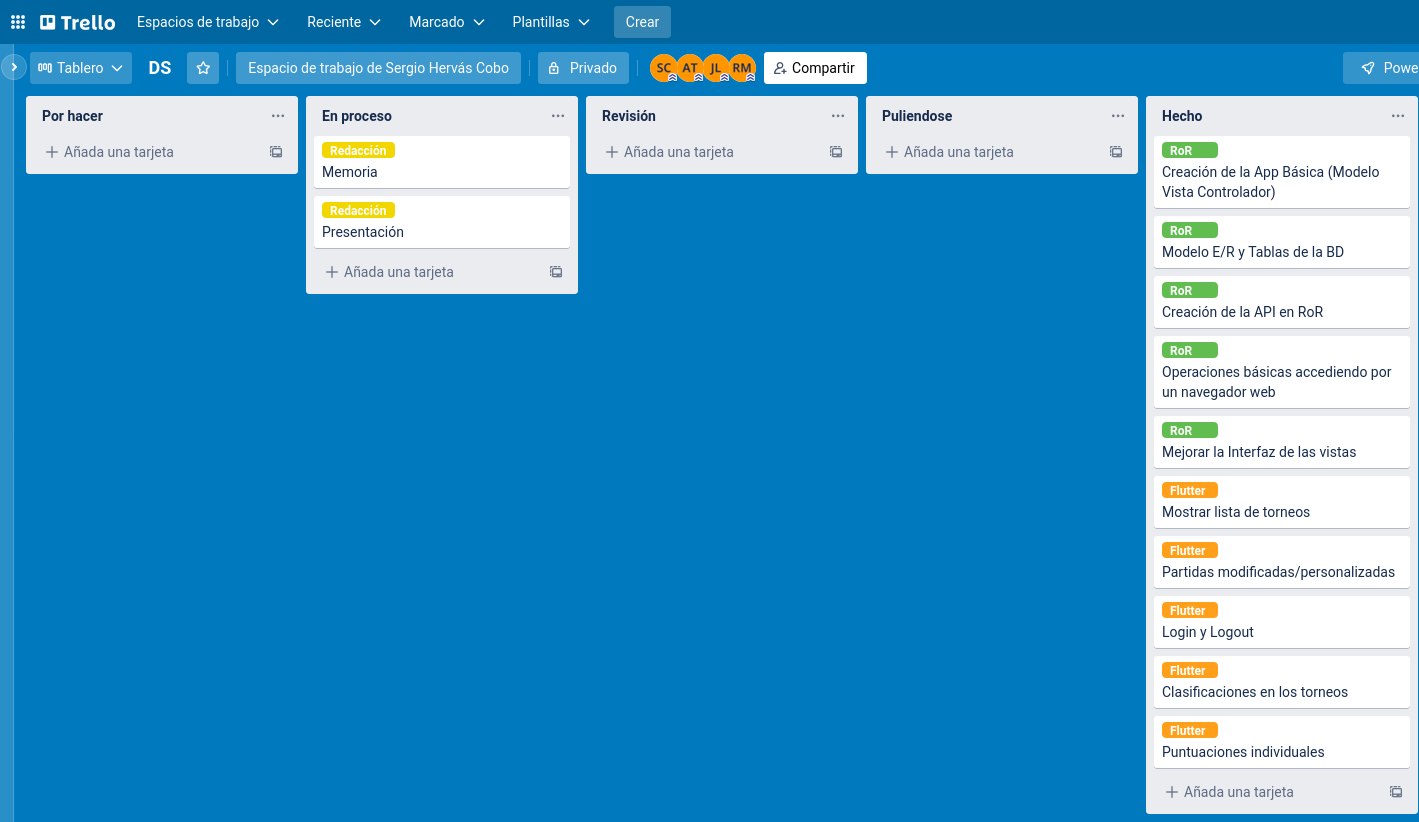
\includegraphics[width=\textwidth]{imagenes/trello.png}
  \caption{Captura de pantalla de nuestro Trello} 
\end{figure}

%\item \textbf{Reparto del trabajo}
\subsection{Reparto del trabajo}

Como ya hemos dicho antes, se han planteado 5 sprints cada equipo aunque la mayoría de sprints han sido realizados de forma bastante grupal entre todos los integrantes.

\begin{table}[H]
  \begin{center}
    \begin{tabularx}{\linewidth}{|X|X|X|} % <-- Alignments: 1st column left, 2nd middle and 3rd right, with vertical lines in between
      \hline
      \textbf{Sprint} & \textbf{Equipo 1} & \textbf{Equipo 2}\\
%      $\alpha$ & $\beta$ & $\gamma$ \\
      \hline
      1 & Planteamos la idea de como va a ser la aplicación y nos organizamos las tareas entre cada equipo & Mejora de la interfaz de las vistas \\
      \hline
      2 & Creación de la App Básica (Modelo Vista Controlador) & Modelo E/R y Tablas de la BD\\
      \hline
      3 & Creación de la API en RoR & Operaciones básicas accediendo por un navegador web\\
      \hline
      4 & Creación de torneos en la App de Flutter & Creación de las puntuaciones en la App de Flutter\\
      \hline
      5 & Creación de partidas configuradas en la App de Flutter & Memoria y Presentación\\
      \hline
    \end{tabularx}
  \end{center}
\end{table}

\section{Fase de análisis}

\subsection {Requisitos Funcionales}
\begin{itemize}
    
    \item RF1 - Interacción con los menús  
    \begin{itemize}
      \item RF1.1 - El sistema debe permitir iniciar la partida.
      \item RF1.2 - El sistema debe permitir salir de la partida y volver a la pantalla de inicio.
      \item RF1.3 - El sistema permitirá a estos usuarios acceder al apartado de créditos. 
      \item RF1.4 - El sistema debe adaptar su apariencia al modo claro u oscuro del dispositivo.
      \item RF1.5 - El sistema debe permitir reanudar la partida desde el menú de pausa.
      \item RF1.6 - El sistema debe permitir salir de la partida y volver al menú principal desde el menú de pausa.
    \end{itemize}

    \item RF2 - Interacción con la partida
    \begin{itemize}
      \item RF2.1 - El sistema debe permitir al usuario manejar el movimiento de las
      piezas (traslación y rotación)
      \item RF2.2 - El sistema debe permitir al usuario reservar una pieza
      \item RF2.3 - El sistema debe permitir pausar la partida en cualquier momento como en reproducción (pararla o reanudarla).
      \item RF2.4 - El sistema debe aumentar la puntuación mediante se van completando filas.
      \item RF2.5 - El sistema debe de subir de nivel tras completar 10 filas.
      \item RF2.6 - El sistema debe de aumentar la velocidad de bajada de las piezas al subir de nivel.
    \end{itemize}

    \item RF3 - Información mostrada durante la partida
    \begin{itemize}
      \item RF3.1 - El sistema debe mostrar la puntuación, el nivel y las filas
      \item RF3.2 - El sistema debe mostrar una lista de piezas siguientes.
      \item RF3.3 - El sistema mostrará un tablero con las piezas que están colocadas y siendo colocada.
    \end{itemize}
    

    \item RF4 - Apartado Musical
    \begin{itemize}
      \item RF4.1 - El usuario podrá desactivar o activar la música.
      \item RF4.2 - El sistema debe de aumentar la velocidad de la música al subir de nivel.
    \end{itemize}

     \item RF5 - Posibilidades de los usuarios no registrados
     \begin{itemize}
      \item RF5.1 - El sistema permitirá jugar partidas normales a estos usuarios pero no guardar su puntuación.
      \item RF5.2 - El sistema permitirá jugar partidas bomba a estos usuarios pero no guardar su puntuación.
    \end{itemize}

    \item RF6 - Posibilidades de los usuarios registrados
     \begin{itemize}
      \item RF6.1 - El sistema permitirá jugar partidas a estos usuarios y guardar su puntuación.
      \item RF6.2 - El sistema permitirá a cada usuario acceder a sus puntuaciones personales.
      \item RF6.3 - El sistema permitirá a estos usuarios poder ver la lista de torneos.
      \item RF6.4 - El sistema permitirá poder ver la información de cada torneo.
      \item RF6.5 - El sistema permitirá jugar los torneos activos que no hayan sido jugados.
      \item RF6.6 - El sistema permitirá ver las puntuaciones guardadas por los participantes del torneo.
      
    \end{itemize}

    \item RF7 - Gestión por administradores
    \begin{itemize}
      \item RF7.1 - El sistema permitirá crear y editar torneos desde la aplicación web.
      \item RF7.2 - El sistema permitirá crear y editar usuarios desde la aplicación web.
      \item RF7.3 - El sistema permitirá crear y editar participaciones desde la aplicación web.

      
    \end{itemize}

    \item RF8 - Gestión de usuarios
    \begin{itemize}
      \item RF8.1 - El sistema permitirá tanto en la aplicación de web como de móvil iniciar sesión si no está activa una.
      \item RF8.2 - El sistema permitirá tanto en la aplicación de web como de móvil cerrar sesión si está activa una.
    \end{itemize}

    

\end{itemize}

\begin{table}[H]
  \begin{center}
    \begin{tabularx}{\linewidth}{|X|X|X|} % <-- Alignments: 1st column left, 2nd middle and 3rd right, with vertical lines in between
      \hline
      \textbf{Detalle} & \textbf{Descripción}\\
%      $\alpha$ & $\beta$ & $\gamma$ \\
      \hline
      RF & 2.3 \\
      \hline
      Nombre & Pausar partida\\
      \hline
      Descripción & El sistema debe permitir pausar la partida en cualquier momento como en reproducción.\\
      \hline
      Entrada & Se pulsa el botón de pausa o se sale de la aplicación.\\
      \hline
      Procesamiento & Coloca en la pila la pantalla de pausa\\
      \hline
      Salida & Pantalla de pausa\\
      \hline
    \end{tabularx}
  \end{center}
\end{table}

\begin{table}[H]
  \begin{center}
    \begin{tabularx}{\linewidth}{|X|X|X|} % <-- Alignments: 1st column left, 2nd middle and 3rd right, with vertical lines in between
      \hline
      \textbf{Detalle} & \textbf{Descripción}\\
%      $\alpha$ & $\beta$ & $\gamma$ \\
      \hline
      RF & 2.1 \\
      \hline
      Nombre & Movimiento de las piezas.\\
      \hline
      Descripción & El sistema debe permitir al usuario manejar el movimiento de las piezas (traslación y rotación)\\
      \hline
      Entrada & Se pulsa el botón de pausa o se sale de la aplicación.\\
      \hline
      Procesamiento & Coloca en la pila la pantalla de pausa\\
      \hline
      Salida & Pantalla de pausa\\
      \hline
    \end{tabularx}
  \end{center}
\end{table}

\begin{table}[H]
  \begin{center}
    \begin{tabularx}{\linewidth}{|X|X|X|} % <-- Alignments: 1st column left, 2nd middle and 3rd right, with vertical lines in between
      \hline
      \textbf{Detalle} & \textbf{Descripción}\\
%      $\alpha$ & $\beta$ & $\gamma$ \\
      \hline
      RF & 2.2 \\
      \hline
      Nombre & Reservar pieza.\\
      \hline
      Descripción & El sistema debe permitir al usuario reservar una pieza\\
      \hline
      Entrada & Pulsación de la tecla para reservar.\\
      \hline
      Procesamiento & Se almacena la pieza que estaba cayendo y se pone una nueva en caída.\\
      \hline
      Salida & La pieza en el recuadro de reservada.\\
      \hline
    \end{tabularx}
  \end{center}
\end{table}

\begin{table}[H]
  \begin{center}
    \begin{tabularx}{\linewidth}{|X|X|X|} % <-- Alignments: 1st column left, 2nd middle and 3rd right, with vertical lines in between
      \hline
      \textbf{Detalle} & \textbf{Descripción}\\
%      $\alpha$ & $\beta$ & $\gamma$ \\
      \hline
      RF & 1.1 \\
      \hline
      Nombre & Iniciar partida.\\
      \hline
      Descripción &  El sistema debe permitir iniciar la partida.\\
      \hline
      Entrada & Se pulsa el botón de Jugar partida\\
      \hline
      Procesamiento &  Se prepara el tablero para el usuario\\
      \hline
      Salida & Tablero de la partida\\
      \hline
    \end{tabularx}
  \end{center}
\end{table}

\begin{table}[H]
  \begin{center}
    \begin{tabularx}{\linewidth}{|X|X|X|} % <-- Alignments: 1st column left, 2nd middle and 3rd right, with vertical lines in between
      \hline
      \textbf{Detalle} & \textbf{Descripción}\\
%      $\alpha$ & $\beta$ & $\gamma$ \\
      \hline
      RF & 2.1 \\
      \hline
      Nombre & Movimiento de las piezas.\\
      \hline
      Descripción & El sistema debe permitir al usuario manejar el movimiento de las piezas (traslación y rotación)\\
      \hline
      Entrada & Se pulsa el botón de pausa o se sale de la aplicación.\\
      \hline
      Procesamiento & Coloca en la pila la pantalla de pausa\\
      \hline
      Salida & Pantalla de pausa\\
      \hline
    \end{tabularx}
  \end{center}
\end{table}

\begin{table}[H]
  \begin{center}
    \begin{tabularx}{\linewidth}{|X|X|X|} % <-- Alignments: 1st column left, 2nd middle and 3rd right, with vertical lines in between
      \hline
      \textbf{Detalle} & \textbf{Descripción}\\
      \hline
      RF & 5.1 \\
      \hline
      Nombre & Jugar partidas sin registrarse.\\
      \hline
      Descripción & El sistema permitirá jugar partidas normales a estos usuarios pero no guardar su puntuación.\\
      \hline
      Entrada & Pulsar el botón de partida normal sin haber iniciado sesión\\
      \hline
      Procesamiento & Se genera el tablero para poder jugar.\\
      \hline
      Salida & El tablero generado junto con las piezas, listo para jugar.\\
      \hline
    \end{tabularx}
  \end{center}
\end{table}

\begin{table}[H]
  \begin{center}
    \begin{tabularx}{\linewidth}{|X|X|X|} % <-- Alignments: 1st column left, 2nd middle and 3rd right, with vertical lines in between
      \hline
      \textbf{Detalle} & \textbf{Descripción}\\
%      $\alpha$ & $\beta$ & $\gamma$ \\
      \hline
      RF & 4.1 \\
      \hline
      Nombre & Control del volumen de la música.\\
      \hline
      Descripción & El usuario puede activar y desactivar el volumen del juego\\
      \hline
      Entrada & Se pulsa el botón de volumen.\\
      \hline
      Procesamiento & Se activa o desactiva la música de acuerdo al estado anterior. \\
      \hline
      Salida & \\
      \hline
    \end{tabularx}
  \end{center}
\end{table}

\begin{table}[H]
  \begin{center}
    \begin{tabularx}{\linewidth}{|X|X|X|} % <-- Alignments: 1st column left, 2nd middle and 3rd right, with vertical lines in between
      \hline
      \textbf{Detalle} & \textbf{Descripción}\\
%      $\alpha$ & $\beta$ & $\gamma$ \\
      \hline
      RF & 7.1 \\
      \hline
      Nombre & Crear Torneo.\\
      \hline
      Descripción & El sistema permitirá a los administradores crear y editar torneos desde la aplicación web.\\
      \hline
      Entrada & Datos del torneo: Nombre del torneo, tipo de partida, fecha límite, probabilidad de bomba, velocidad de juego y número de bloques iniciales.\\
      \hline
      Procesamiento & Se añade un nuevo torneo a la base de datos\\
      \hline
      Salida & Mensaje de éxito o de error\\
      \hline
    \end{tabularx}
  \end{center}
\end{table}

\begin{table}[H]
  \begin{center}
    \begin{tabularx}{\linewidth}{|X|X|X|} % <-- Alignments: 1st column left, 2nd middle and 3rd right, with vertical lines in between
      \hline
      \textbf{Detalle} & \textbf{Descripción}\\
      \hline
      RF & 6.5 \\
      \hline
      Nombre & Jugar torneo.\\
      \hline
      Descripción & El sistema permitirá jugar los torneos activos que no hayan sido jugados.\\
      \hline
      Entrada & Se pulsa el botón de jugar partida.\\
      \hline
      Procesamiento & Se prepara el tablero de la partida del torneo para el usuario con los parámetros del torneo.\\
      Salida & Tablero del torneo\\
      \hline
    \end{tabularx}
  \end{center}
\end{table}

\begin{table}[H]
  \begin{center}
    \begin{tabularx}{\linewidth}{|X|X|X|} % <-- Alignments: 1st column left, 2nd middle and 3rd right, with vertical lines in between
      \hline
      \textbf{Detalle} & \textbf{Descripción}\\
%      $\alpha$ & $\beta$ & $\gamma$ \\
      \hline
      RF & 6.3 \\
      \hline
      Nombre & Tablero del torneo.\\
      \hline
      Descripción & El usuario podrá ver la lista de torneos disponibles\\
      \hline
      Entrada & Se pulsa el botón de “Torneos”.\\
      \hline
      Procesamiento & Obtiene los torneos del servidor web y los imprime en la app.\\
      \hline
      Salida & Se muestra una tabla interactiva de los torneos abiertos y los torneos finalizados\\
      \hline
    \end{tabularx}
  \end{center}
\end{table}

\begin{table}[H]
  \begin{center}
    \begin{tabularx}{\linewidth}{|X|X|X|} % <-- Alignments: 1st column left, 2nd middle and 3rd right, with vertical lines in between
      \hline
      \textbf{Detalle} & \textbf{Descripción}\\
      \hline
      RF & 6.6 \\
      \hline
      Nombre & Ver los resultados de un torneo.\\
      \hline
      Descripción & El sistema permitirá ver las puntuaciones guardadas por los participantes del torneo.\\
      \hline
      Entrada & Se pulsa sobre el botón de clasificaciones del torneo elegido.\\
      \hline
      Procesamiento & \\
      \hline
      Salida & Tabla con el nombre y la puntuación en orden descendente de las puntuaciones guardadas en el torneo.\\
      \hline
    \end{tabularx}
  \end{center}
\end{table}

\begin{table}[H]
  \begin{center}
    \begin{tabularx}{\linewidth}{|X|X|X|} % <-- Alignments: 1st column left, 2nd middle and 3rd right, with vertical lines in between
      \hline
      \textbf{Detalle} & \textbf{Descripción}\\
      \hline
      RF & 2.2 \\
      \hline
      Nombre & Reserva de piezas.\\
      \hline
      Descripción & El sistema debe permitir al usuario reservar una pieza.\\
      \hline
      Entrada & Se pulsa el botón reserva.\\
      \hline
      Procesamiento & Se quita la pieza actual del tablero, se almacena en reservada y se escoge una nueva.\\
      \hline
      Salida & La pieza antigua en el cajón de reservados y una pieza nueva que irá cayendo.\\
      \hline
    \end{tabularx}
  \end{center}
\end{table}

\subsection{Requisitos No Funcionales}
\begin{itemize}
  \item Aplicación móvil
  \begin{itemize}
    \item El sistema debe trabajar en tiempo real para evitar inconsistencias.
    \item El sistema tendrá una interfaz para el menú para elegir modos y comenzar la partida.
    \item La aplicación cliente está implementado en Dart con Flutter.
    \item Las físicas del sistema no deben estar unidas a los fotogramas por segundo (FPS).
    \item Existirá un modo oscuro que cambie los colores de la interfaz.
    \item Los tipos de datos serán validados por la aplicación 
    \item Las fechas de los torneos serán validadas por la aplicación
  \end{itemize}
  \item Aplicación web
  \begin{itemize}
    \item Los datos se almacenarán en una base de datos relacional, concretamente MySQL.
    \item El servidor web- estará implementado sobre Ruby On Rails
    \item El tiempo de respuesta de las operaciones deberá ser mínimo
    \item Los botones de la aplicación serán lo suficientemente grandes y fáciles de detectar e interaccionar con ellos.
\end{itemize}
\end{itemize}
\subsection{Criterios de calidad} 
\begin{itemize}
  \item Aplicación móvil
  \begin{itemize}
    \item Los movimientos de las piezas deberán verse en pantalla en tiempo real. \textbf{(Usabilidad y Eficiencia)}.

    \item Las colisiones entre piezas se realizan de forma consistente con independencia de la cantidad de bloques que haya en el tablero. \textbf{(Integridad)}.

    \item La puntuación del usuario se actualizará de forma dinámica y correctamente de acuerdo a las reglas preestablecidas. \textbf{(Integridad)}.
    
    \item Que varios usuarios de forma concurrente puedan acceder a la página de torneos. \textbf{(Escalabilidad)}.

    \item Que la aplicación sea fluida en rendimiento en cualquier smartphone Android. \textbf{(Eficiencia)}
    
    \item Que la información que se inserta en el servidor web aparezca correctamente en la aplicación. \textbf{(Integridad)}
   
    \item Que la aplicación móvil sea responsive en cualquier smartphone Android. \textbf{(Usabilidad)}
  \end{itemize}
  \item Aplicación web
  \begin{itemize}
    \item Que la aplicación web sea responsive en cualquier dispositivo (ordenadores, móviles, tabletas...) \textbf{(Usabilidad)}.

    \item Que la aplicación web sea sencilla, intuitiva y fácil de manejar \textbf{(Usabilidad)}

    \item Que los usuarios no administradores no puedan acceder a la gestión de torneos o usuarios o a cualquier sitio de la web no autorizado. \textbf{Seguridad}

    \item Que los usuarios no administradores no pueden acceder a la información de otros usuarios. \textbf{Seguridad}
    
    \item La inserción, modificación y el borrado de una tupla en la base de datos no ocasionará problemas de inexistencia o falta de información. \textbf{(Integridad)}

    \item Que la interacción con los distintos botones de la página web no de problemas en cuanto al tamaño o la percepción de estos \textbf{(Accesibilidad)}
  \end{itemize}
\end{itemize}

\subsection{Diagramas}
\subsubsection{Diagrama de contexto}
Para el diagrama de contexto, se han definido los cuatro subsistemas que hay en nuestras aplicaciones:
\begin{itemize}
\item Subsistema de usuarios: Registro y login del cliente.  
\item Subsistema de torneos: Partidas personalizadas creadas por el staff del sistema y las cuales los usuarios podrán jugar. 
\item Subsistema de puntuaciones: Las partidas individuales serán tratadas para que el usuario pueda ver todas sus puntuaciones
\item Subsistema de juego: Es la funcionalidad básica del juego "Haz Una Línea".
\end{itemize}

Además, también se ha representado la base de datos que almacenará el modelo que utilizarán los subsistemas anteriores.
  \begin{figure}[H]
  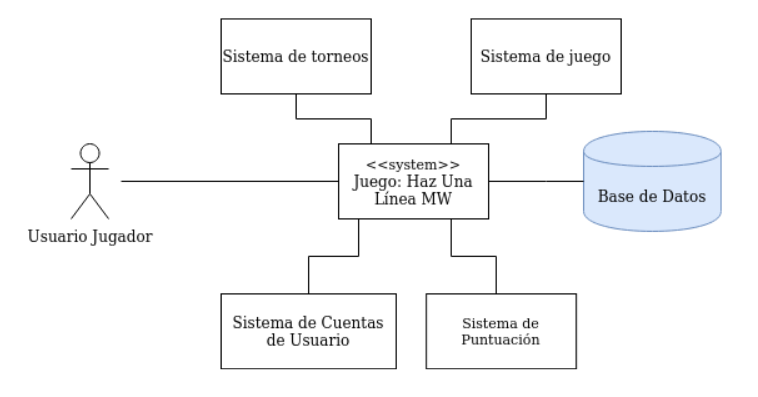
\includegraphics[width=\textwidth]{imagenes/contexto.png}
  \caption{Diagrama de clases de la aplicación} 
\end{figure}

\subsubsection{Diagrama de paquetes}
%PONER DIAGRAMA DE PAQUETES
A continuación se muestra el diagrama de paquetes de la aplicación del lado del cliente. Consta de los siguientes paquetes:

\begin{itemize}
  \item \textbf{pantallas: }Distintas pantallas de la app.
  \item \textbf{Factoria: }Distintos algoritmos de creación de piezas.
  \item \textbf{main: }Funcionalidad principal.
  \item \textbf{Piezas: }Todas las piezas del juego.
  \item \textbf{api: }Interfaz para la conexión con el servidor.
\end{itemize}

\begin{figure}[H]
  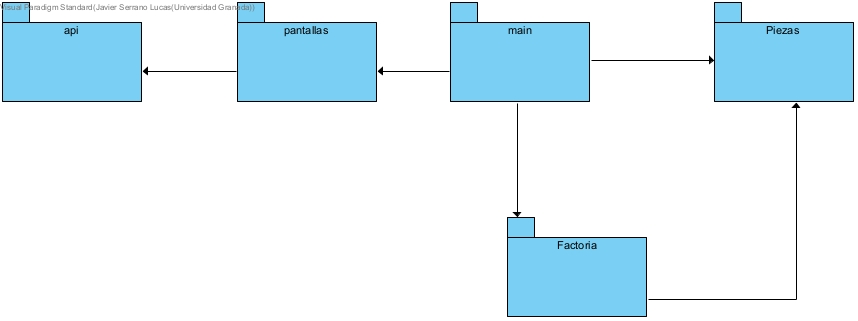
\includegraphics[width=\textwidth]{imagenes/DiagramaPaquetes2.jpg}
  \caption{Diagrama de paquetes de la aplicación del cliente} 
\end{figure} 

\subsubsection{Modelo E/R}
A continuación, mostramos los distintos elementos que habrá en nuestra base de datos y sus atributos que especificarán las características de cada uno.
\begin{figure}[H]
  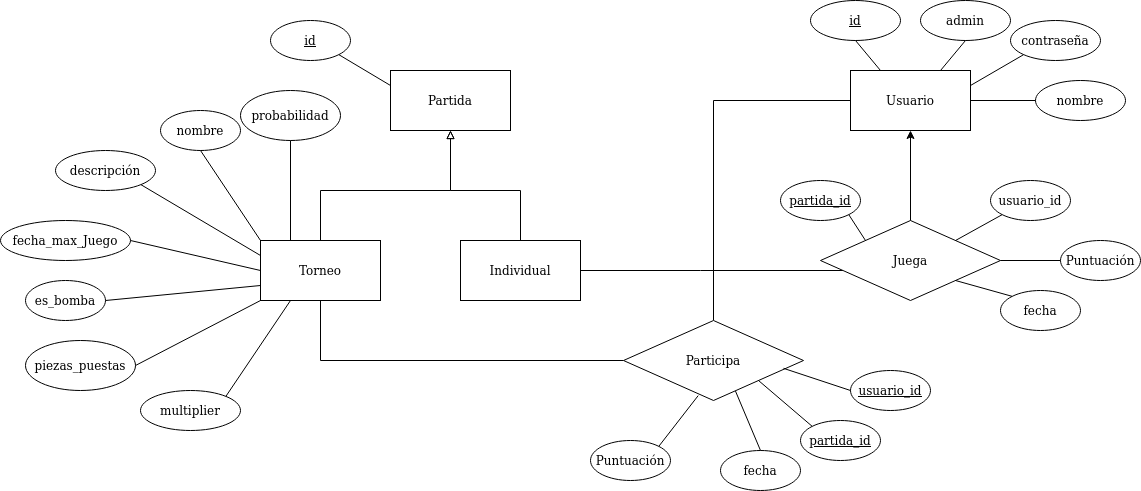
\includegraphics[width=\textwidth]{imagenes/er.png}
  \caption{Diagrama del modelo E/R de nuestro sistema} 
\end{figure} 


\subsection{Partes Interesadas}

\begin{itemize}
    \item \textbf{Usuario}: Es el jugador que utiliza la aplicación desarrollada. En nuestro caso, juega al videojuego.
    \item \textbf{Equipo de prueba}: Son los encargados de ejecutar los ficheros de prueba, y de realizar tests sobre
    la aplicación tras una actualización antes de lanzar la nueva versión para todo el público.
    \item \textbf{Desarrollador}: Es el encargado de crear e implementar el código del videojuego.
    \item \textbf{Usuario Organizador (Moderador)}: Se encargará de crear torneos nuevos en la web.
    \item \textbf{Administrador}: Se encarga de que los torneos sean correctos y del buen funcionamiento del servidor.
    \item \textbf{Mantenedores}: Son los encargados de hacer los mantenimientos para aplicar las nuevas actualizaciones de una manera rápida, y también que cuando el sistema falle, puedan dar con una solución rápida.
    \item \textbf{Ingenieros de producción}: Es el encargado de diseñar y crear un servidor y una base de datos, de una manera que no se sature con demasiada facilidad.
    \item \textbf{Equipo de apoyo}: Son los encargados de velar por una experiencia satisfactoria en el juego de todos los usuarios, mediante arreglar problemas, bugs, y demás en foros, o en el Discord del juego (Son unos usuarios que han cogido ese rol dentro de la comunidad).
\end{itemize}

\subsection{Diseño de Pruebas de Sistema e Integración}

\subsubsection{Pruebas P3}

\begin{itemize}
    \item Pruebas de Unidad
    \begin{itemize}
      \item El volumen de la música debería cambiar a 0: Se comprobará que el volumen de la música es 0 cuando se pulse el botón del volumen.
    
      \item El volumen de la música debería cambiar a 1: Se comprobará que el volumen de la música es 1 cuando se pulse el botón del volumen.
      
      \item La pieza no se debe mover en los bordes del tablero: Este test verifica si al mover una pieza que está en el borde del tablero en esa misma dirección, esta permanece en el mismo sitio sin salirse del tablero. El test se dará como correcto si todas las piezas no se salen del tablero tanto por la izquierda como por la derecha
      
      \item La bomba explota: Este test se encargará de comprobar que las piezas bombas al detonar eliminan los bloques colindantes y los propios bloques de la pieza bomba.Se dará como correcto si los bloques del tablero de alrededor de la bomba y los de la propia pieza bomba son nulos.
      
      \item La pieza está en el suelo: Este test comprobará que la pieza al bajarla se encuentre en el suelo del tablero y no haya bajado más de la cuenta.
  
      \item Todas las piezas creadas son distintas: Este test comprueba que el algoritmo usado en la factoría para obtener las piezas es consistente. Se dará como correcto el test si al sacar el mismo número de piezas que las pasadas a la factoría al final son todas distintas.
    
      \item La pieza detecta colisión con otra de abajo: Este test se encarga de comprobar que al poner una pieza encima de otra no la atraviese y detecte correctamente la colisión.
  
      \item Cuando se forman 10 bloques horizontales se destruye una línea: Este test consiste en colocar 10 bloques (en este caso 5 cubos) y comprobar que al hacer la línea (2 en esta ocasión) se eliminan del tablero.
    \end{itemize}
    \item Pruebas de Widgets
    \begin{itemize}
    \item Cambio de icono al apagar/encender la música: Se comprobará si el icono del altavoz se alterna al apretarlo para cambiar el volumen de la música
    
    \item Aparece la pantalla de Game Over: Se comprueba si al pasar un tiempo, el juego termina por la llegada de las piezas a la parte superior del tablero.

    \item Al salir de la partida desde el menú de pausa regresa al menú principal: Se verifica que al pulsar el botón de salir en la pantalla Pause se vuelve a la pantalla de inicio.
    
    \item Al reservar la pieza, esta aparece en la pantalla: Se comprueba si al pulsar ``Guardar'' por primera vez, la pieza actual pasa a ser una pieza reservada.
  \end{itemize}
\item Pruebas de integridad: La prueba de Widgets ``Game Over'' podría ser considerada de integridad.

  \end{itemize}

\subsubsection{Pruebas P4 en RoR}

\begin{itemize}
    \item Test Fixtures 1: Un usuario creado tiene el nombre esperado.

    \item Test Fixtures 2: Un usuario creado tiene el id esperado.
    
    \item Test Modelos 1: Un usuario creado no es admin por defecto.

    \item Test Integración 1: Se puede acceder correctamente a la página para crear torneos por el método GET y se puede crear un torneo con el método POST. Redirige correctamente a otra página donde se encuentra un mensaje de éxito
    
    \item Test Integración 2: Se puede acceder correctamente a la página para crear usuarios por el método GET y se puede crear un usuario con el método POST. Redirige correctamente a otra página donde se encuentra un mensaje de éxito
\end{itemize}

\begin{figure}[H]
  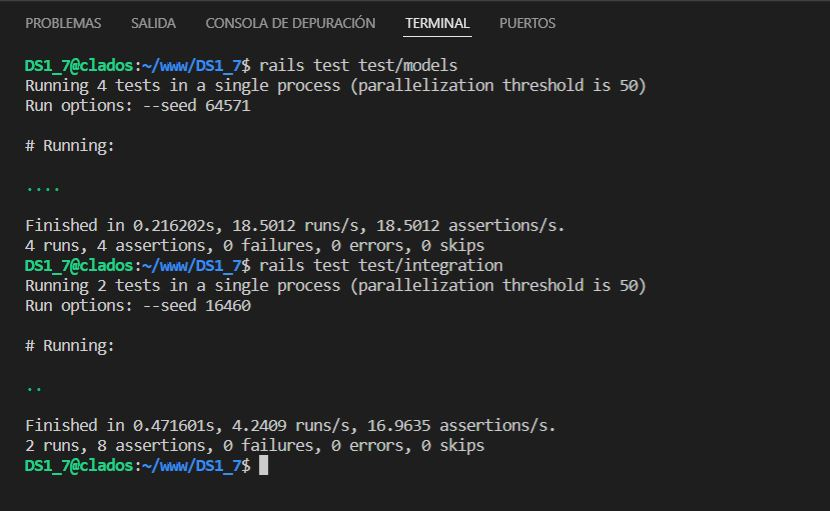
\includegraphics[width=\textwidth]{imagenes/Pruebas.JPG}
  \caption{Salida de la ejecución de todas las pruebas realizadas para Ruby on Rails} 
\end{figure}

\section{Fase de diseño}
\subsection{Diagrama de clases}
La aplicación se ha dividido en varios paquetes para poder encapsular la funcionalidad similar:

\begin{itemize}
  \item \textbf{Pieza: }Paquete de la izquierda, contiene todo lo relativo a las piezas que la aplicación tiene. La clase Pieza se encarga de aportar a sus hijos la funcionalidad principal (colisiones, movimientos y giros). Esta clase contiene un conjunto de bloques, que son los que finalmente se pondrán en el tablero y los que le dan forma a la pieza.
  \item \textbf{Factoria: }Paquete que se encarga de generar las piezas siguiendo las normas del Tetris original. Está formado por dos implementaciones concretas, ``FactoriaConcreta'', usada para el juego normal, y ``FactoriaConcretaEspecial'', usada para generar las piezas normales y según una probabilidad, generar piezas bomba.
  \item \textbf{Main: }Este paquete tiene la funcionalidad del propio tablero y sus parámetros. El tablero es la pantalla propia del juego, que implementa las reglas y funcionalidad propias del tablero y usa los métodos de las piezas. ``ParametrosTablero'' se encarga de almacenar la configuración del tablero y, en esta práctica, también cierto estado sobre la aplicación (si el usuario ha iniciado sesión, está en un torneo, etc).
  \item \textbf{Pantalla: }Implementa las distintas pantallas de la aplicación, no tienen lógica muy compleja, excepto para las pantallas de esta práctica, que varían según el estado de la aplicación.
  \item \textbf{api: }Este paquete implementa la interfaz que se conecta con el servidor web para realizar peticiones y enviar información a la misma. Es el que se encarga de obtener los torneos, credenciales de usuario, puntuaciones individuales y de torneo, etc.
\end{itemize}


\begin{figure}[H]
  \includegraphics[width=\textwidth]{imagenes/clase_final.png}
  \caption{Diagrama de clases de la aplicación} 
\end{figure}

\section{Fase de codificación}
A continuación detallaremos el proceso de desarrollo junto con los problemas que hemos ido teniendo al realizar la práctica

Para empezar, lo primero que hicimos fue plantear el modelo (la base de datos). Para ello, creamos un modelo E/R que reflejase las tablas y las relaciones entre ellas
que queríamos tener. Una vez decidimos la estructura final de la base de datos, realizamos el paso a tablas y la fusión de estas para poder crear las tablas en Ruby.

Cuando ya teníamos la estructura de los datos que queríamos almacenar, creamos los Scaffolds de Ruby on Rails en la aplicación que teníamos por defecto creada. Así, ya teníamos el 
modelo, la vista y el controlador bien separados y definidos en los directorios. Aquí tuvimos unos cuantos problemas, ya que teníamos que destruir todos los Scaffolds cada vez que queríamos
modificar algo del modelo. Al final realizamos un script que automatizase todos los comandos que debíamos poner para realizar algún cambio en la base de datos.

Posteriormente, creamos la API para la conexión con los clientes de la aplicación. Para ello, tuvimos que crear una API para los torneos, usuarios, puntuaciones individuales y puntuaciones del torneo. Cada una implementa la funcionalidad necesaria para obtener la información que se necesita en cada momento, por ejemplo, para los torneos, se implementa show, que muestra un torneo concreto con la id pasada como parámetro en la URL, mientras que en index muestra todos los torneos, incluyendo información adicional extraída con sentencias SQL. 

Un problema que tuvimos a la hora de implementarlo es que solo se podía pasar un parámetro en la URL y no encontramos forma sencilla de arreglarlo. Al final optamos por usar el único parámetro para buscar por otros campos, en vez de usarlo para la id, como tiene RoR por defecto. 

Otro problema que tuvimos era, como RoR principalmente usa métodos para filtrar los registros de la base de datos, no podíamos realizar consultas más complejas. Al final la solución fue usar el método ``exec\_query'' para poder obtener la información deseada usando SQL.

Una vez preparada la API en Ruby On Rails, nos pusimos manos a la obra con la funcionalidad en Flutter. Para ello añadimos un botón que permitiese entrar a los torneos. Una vez hecho esto, los usuarios
podrán acceder a los torneos. Se accedió a la API para listar todos los torneos existentes, para crear una participación a un torneo y una jugada en una partida individual.
En este caso, se nos hizo un poco cuesta arriba la conexión con la API por diversos fallos que tuvimos, como por ejemplo los tipos de datos que recibía del servidor, el nombre
de los atributos del Json, etc.

Por último, se añadió la funcionalidad a Ruby On Rails. Por cada pantalla había que crear una nueva vista, un nuevo controlador y añadir la configuración al fichero de rutas.
\begin{itemize}
  \item Creamos el login y el registro en el servidor web. Para ello, tuvimos que aprender a usar ciertas sentencias
de RoR como la asignación a la variable ``session'' para mantener la sesión iniciada o el acceso a los hiperenlaces a las distintas rutas del servidor web.  
  \item Creamos la lista de torneos: Para ello utilizamos el bucle for en rails incrustado en HTML
  \item Creamos la lista de puntuaciones individuales: Se hizo de la misma forma que el punto anterior
  \end {itemize}

Una vez teníamos toda la lógica implementada, solo faltaba la estética de la aplicación. Hemos decidido optar por un diseño simple pero intuitivo y minimalista. Por ello,
simplemente realizamos. Mediante un fichero CSS, se dieron ciertas reglas para cambiar el formato y el estilo de los distintos elementos del sitio web.

\section{Fase de pruebas}
\begin{itemize}
  \item \textbf{Test Fixtures 1: Un usuario creado tiene el nombre esperado.}
  Se comprobará si un usuario que se ha registrado tiene su nombre almacenado correctamente, es decir,
  si es igual al que tiene en la base de datos.

  Se dará como correcto el test si las dos cadenas de caracteres coinciden.

  \item \textbf{Test Fixtures 2: Un usuario creado tiene el id esperado.}
  Se comprobará si un usuario que se ha registrado tiene su id almacenado correctamente, es decir,
  si es igual al que tiene en la base de datos. 

  Se dará como correcto el test si los dos números enteros del id coinciden.

  \item \textbf{Test Modelos 1: Un usuario creado no es admin por defecto.}
  Se comprobará si un nuevo usuario no tiene el rol de administrador por defecto. Es decir,
  el campo de admin tiene que ser falso cuando se crea el usuario.

  Se dará como correcto el test si el campo ``admin'' del usuario es 0.

  \item \textbf{Test Integración 1: Gestión de torneos} Se comprobará si se puede acceder correctamente a la página para crear torneos por el método GET y
   se puede crear un torneo con el método POST. Redirige correctamente a otra página donde se encuentra un mensaje de éxito.

   Se dará correcto si encuentra el texto de que se ha creado el torneo correctamente
   \item \textbf{Test Integración 2: Gestión de usuarios} Se comprobará si se puede acceder correctamente a la página para crear usuarios por el método GET y
   se puede crear un usuario con el método POST. Redirige correctamente a otra página donde se encuentra un mensaje de éxito.

   Se dará correcto si encuentra el texto de que se ha creado el usuario correctamente

\end{itemize}

\section{Capturas de pantalla}
A continuación, vamos a adjuntar algunas capturas de pantalla de muchas de las secciones que hemos realizado para esta práctica, tanto en la aplicación móvil como en el sitio web.
\subsection{Aplicación móvil}
\begin{figure}[H]
  \centering
  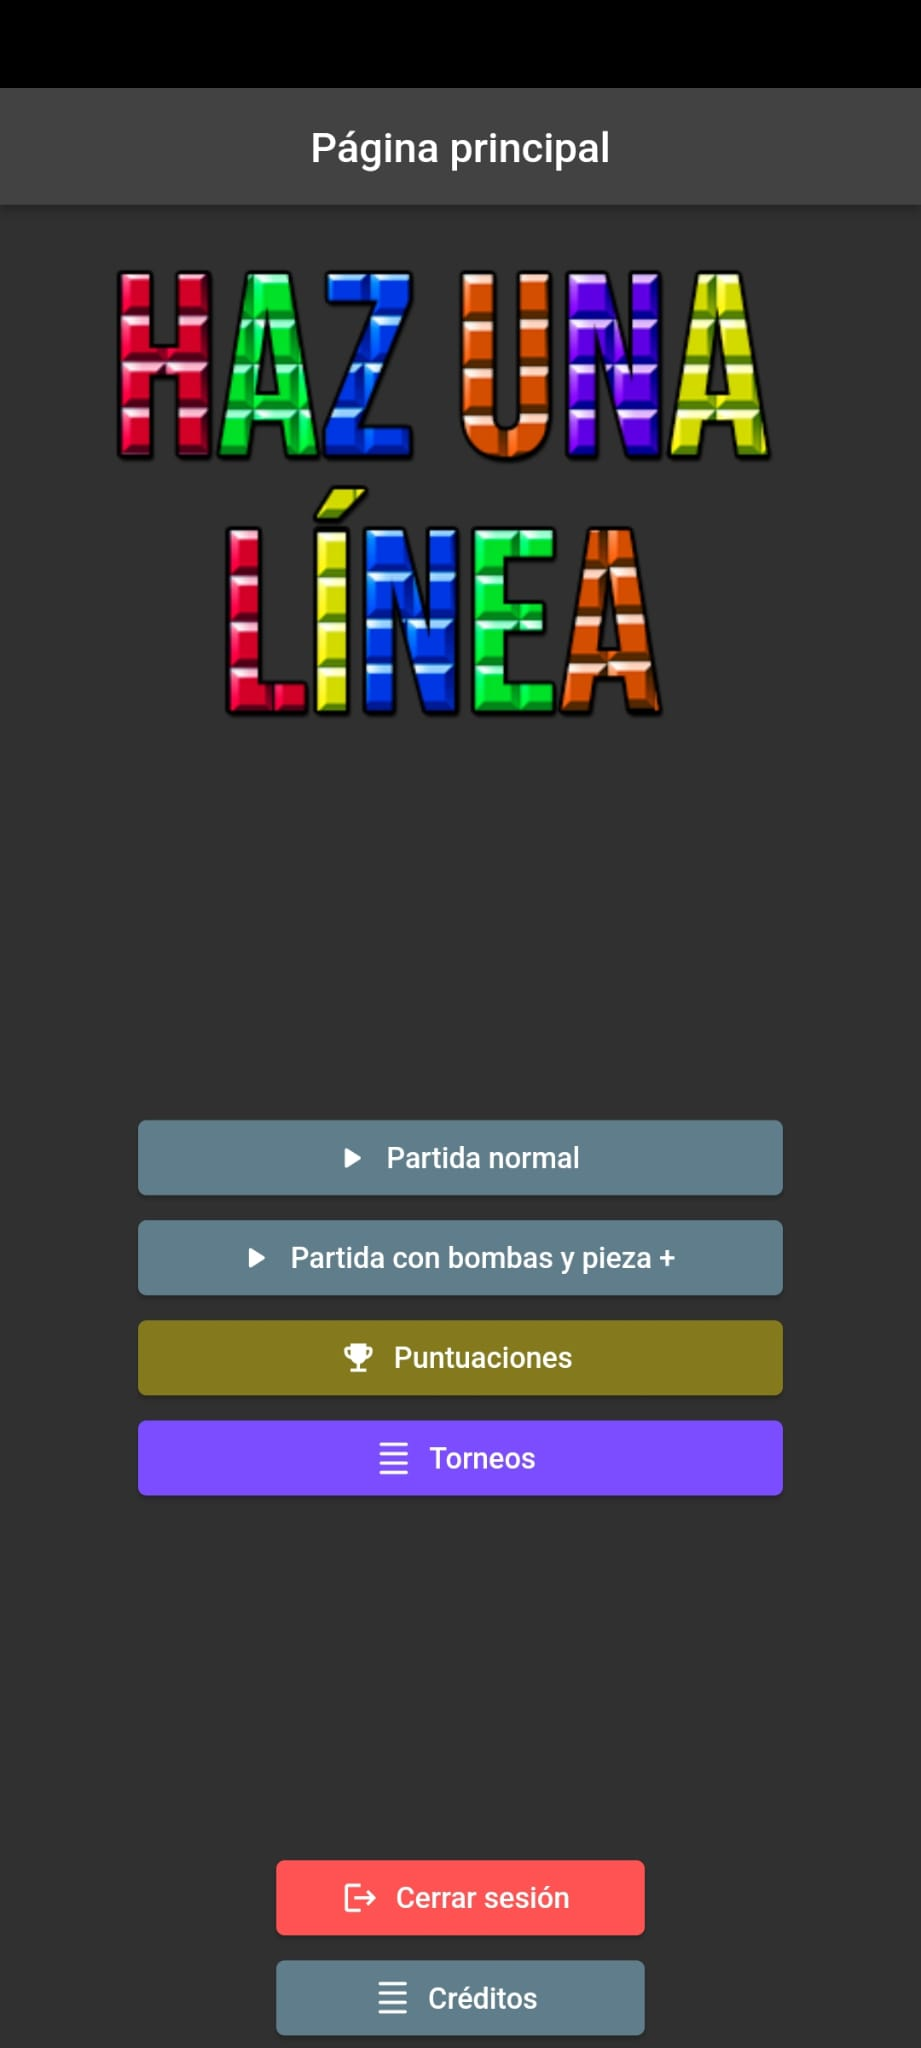
\includegraphics[width=0.5\textwidth]{imagenes/inicio.jpeg}
  \caption{Pantalla principal} 
\end{figure} 

\begin{figure}[H]
  \centering
  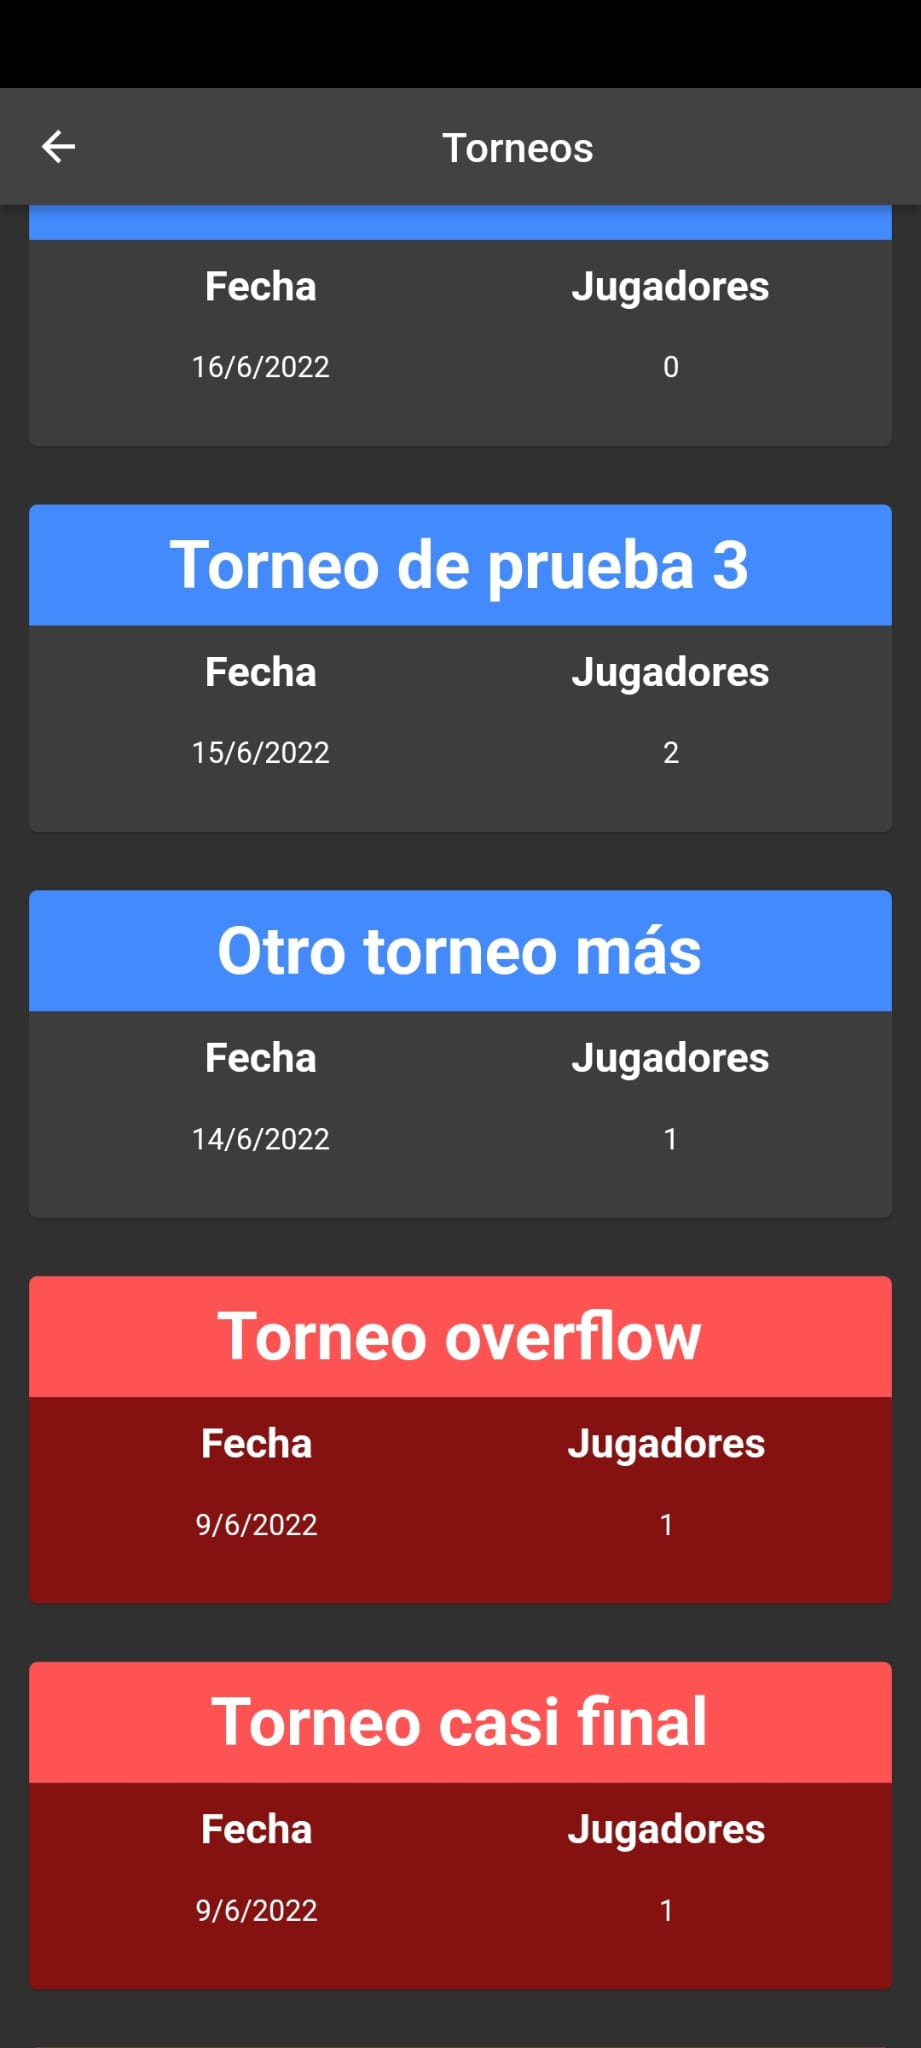
\includegraphics[width=0.5\textwidth]{imagenes/torneos.jpeg}
  \caption{Sección de torneos} 
\end{figure} 

\begin{figure}[H]
  \centering
  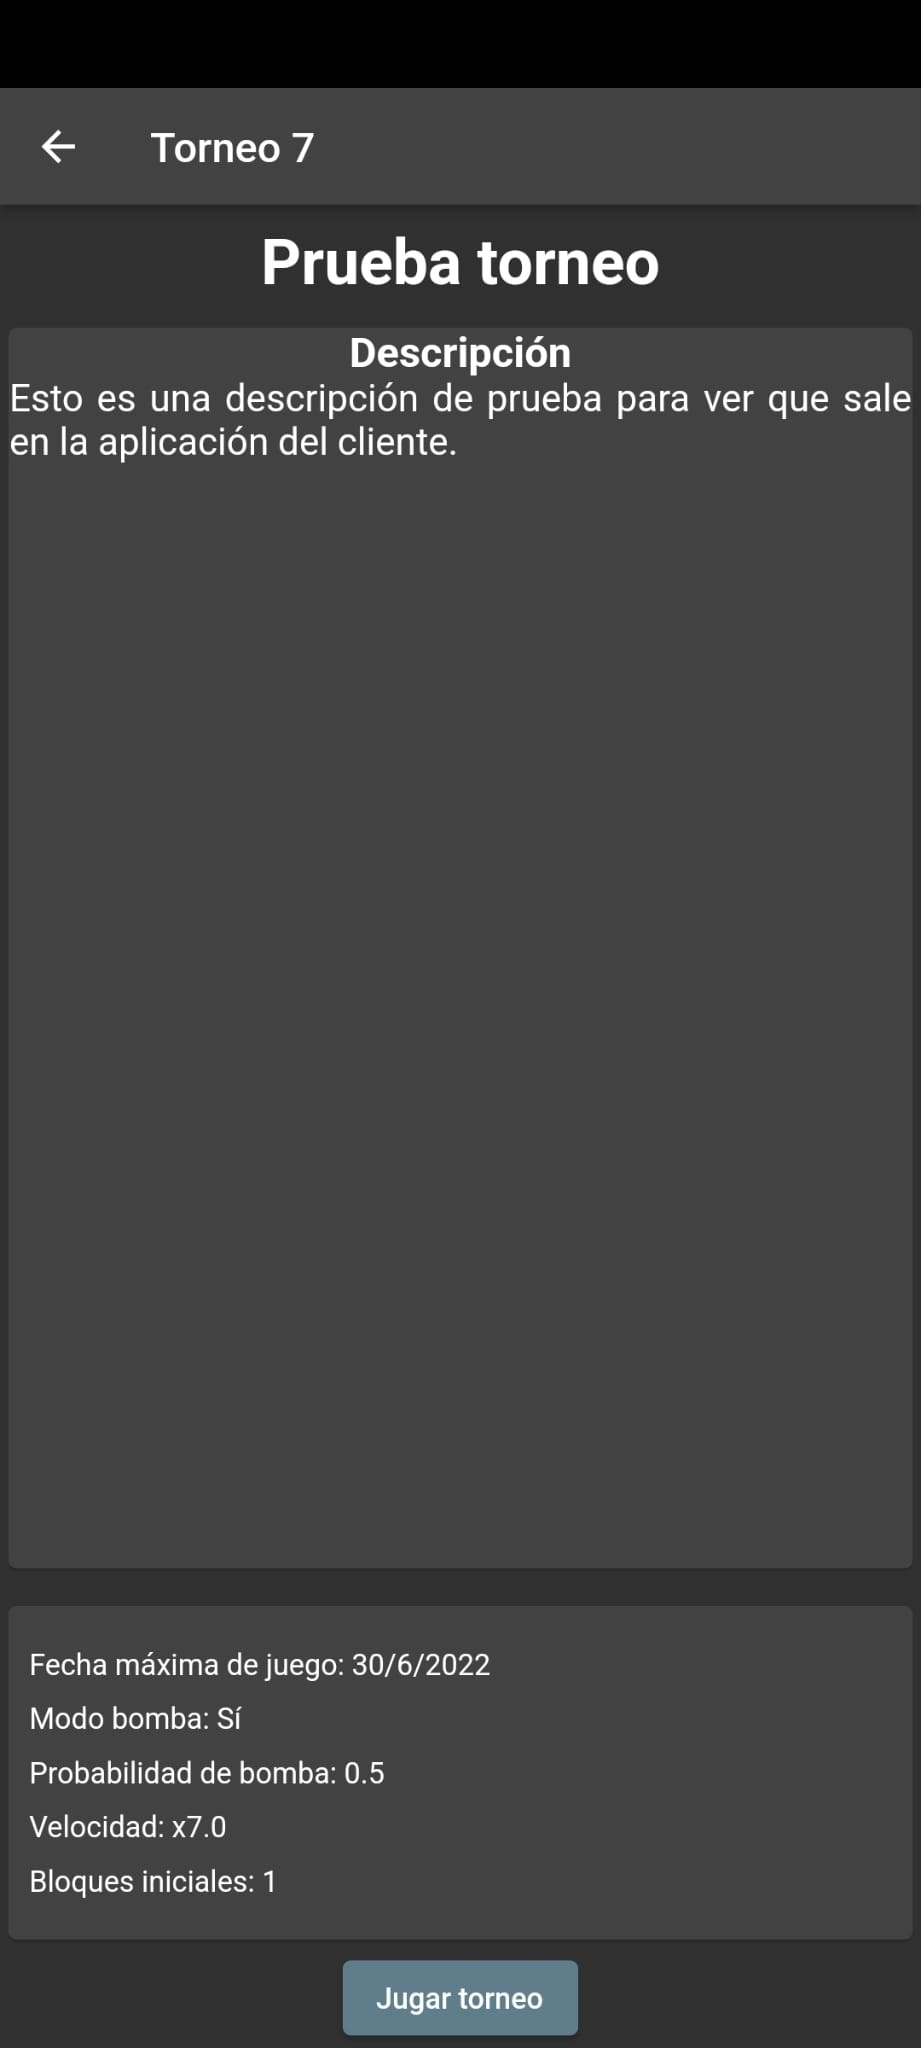
\includegraphics[width=0.5\textwidth]{imagenes/torneo.jpeg}
  \caption{Información de un torneo} 
\end{figure} 

\begin{figure}[H]
  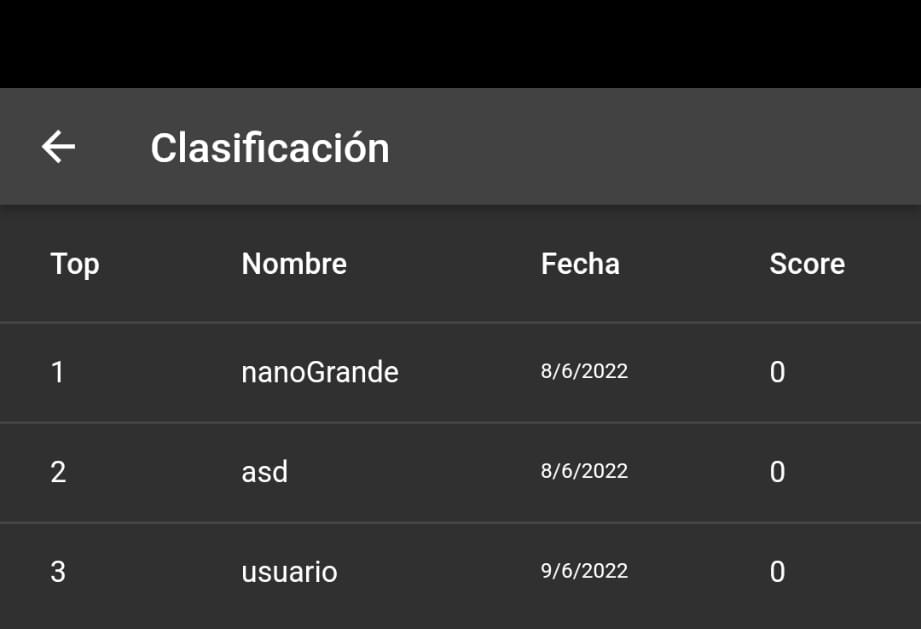
\includegraphics[width=\textwidth]{imagenes/clasTorneo.jpeg}
  \caption{Clasificación de un torneo} 
\end{figure} 

\begin{figure}[H]
  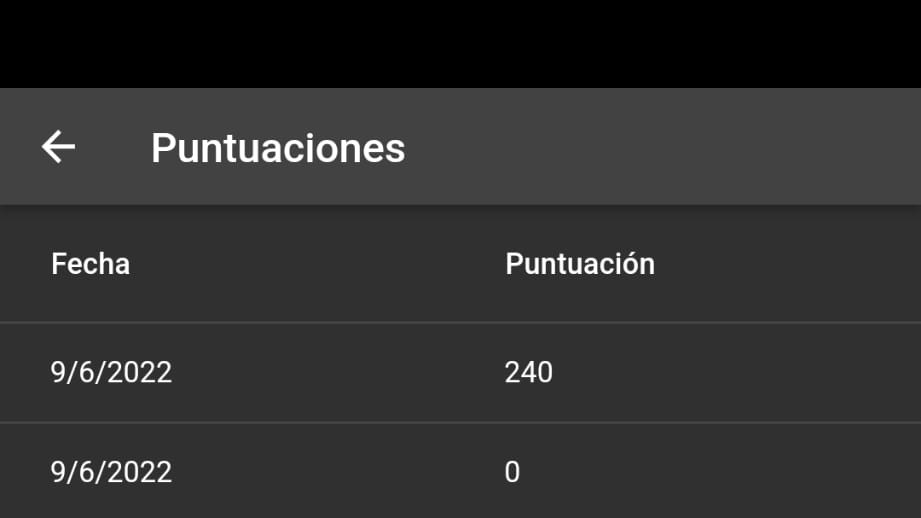
\includegraphics[width=\textwidth]{imagenes/clasInd.jpeg}
  \caption{Puntuaciones de un usuario} 
\end{figure} 

\begin{figure}[H]
  \centering
  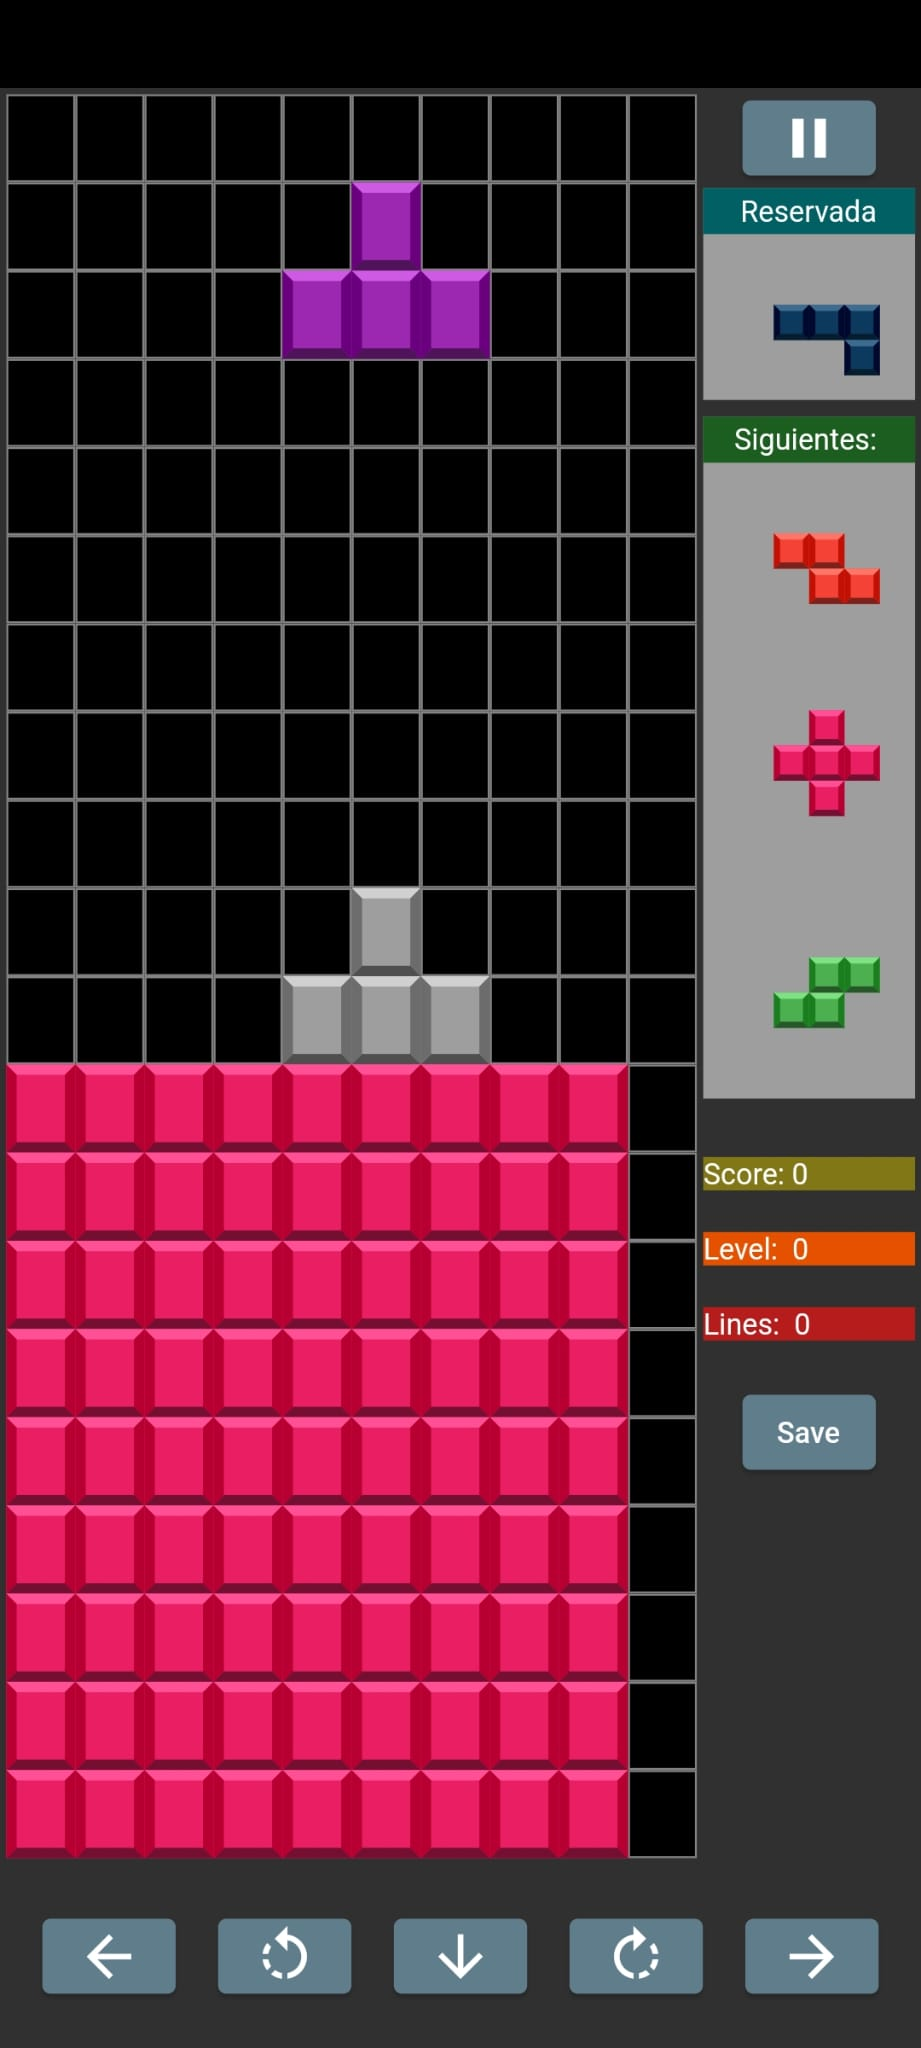
\includegraphics[width=0.5\textwidth]{imagenes/piezasRosas.jpeg}
  \caption{Partida personalizada de un torneo} 
\end{figure}

\subsection{Aplicación web}
\begin{figure}[H]
  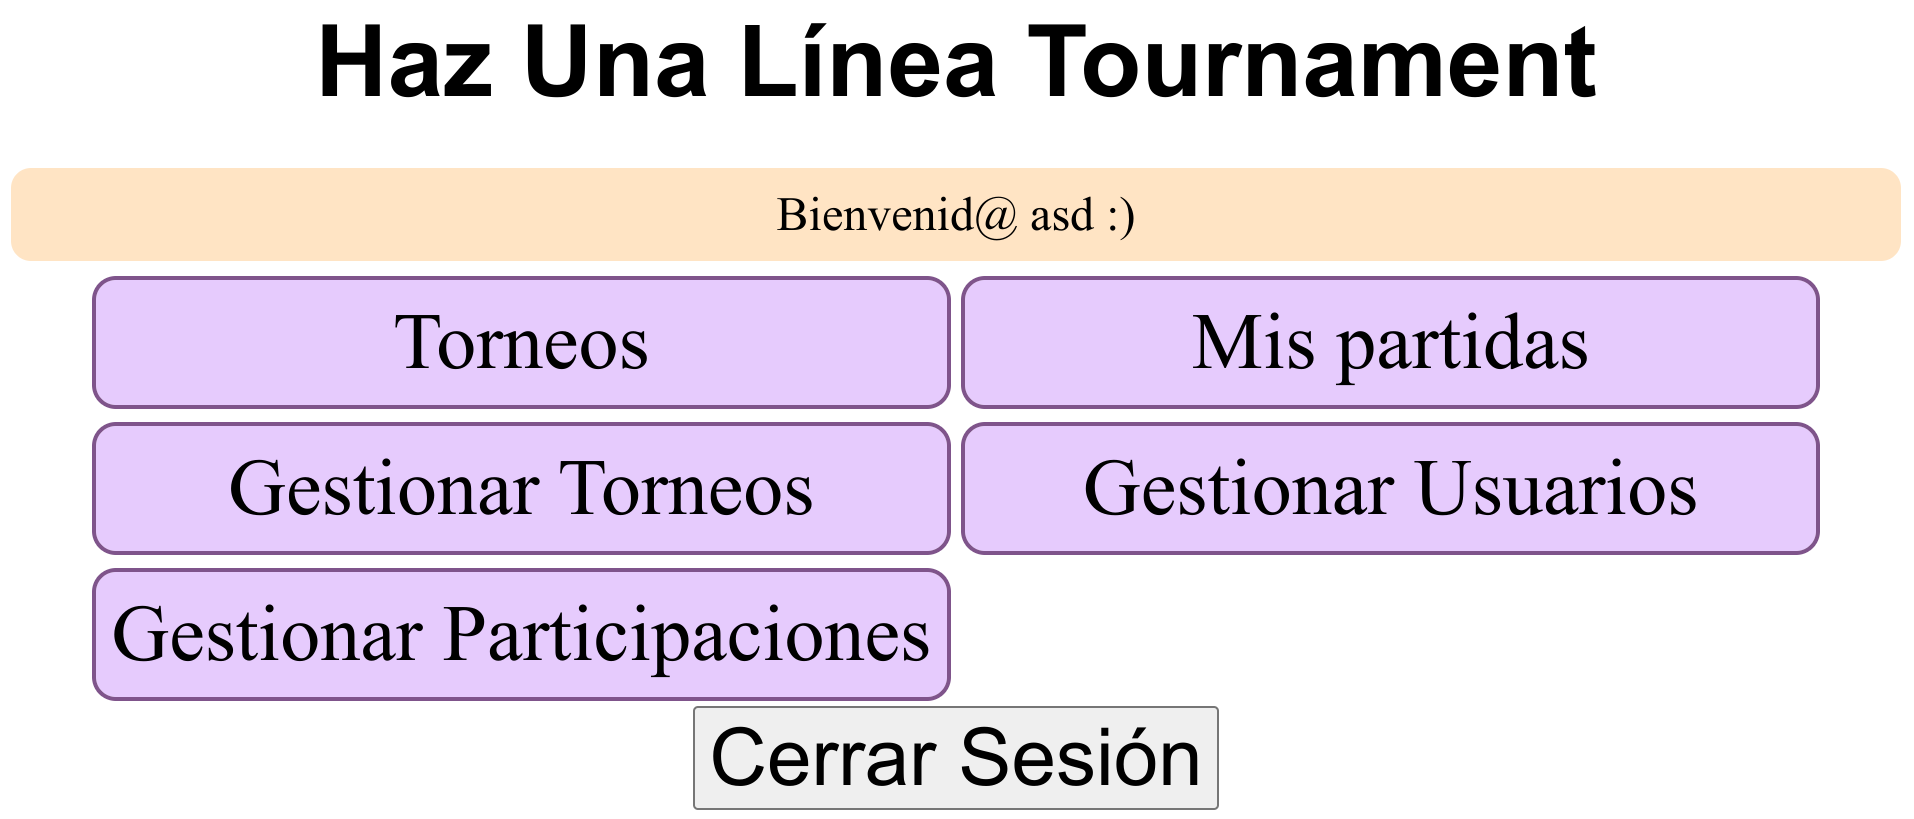
\includegraphics[width=\textwidth]{imagenes/inicioAdmin.png}
  \caption{Página de inicio del administrador} 
\end{figure}

\begin{figure}[H]
  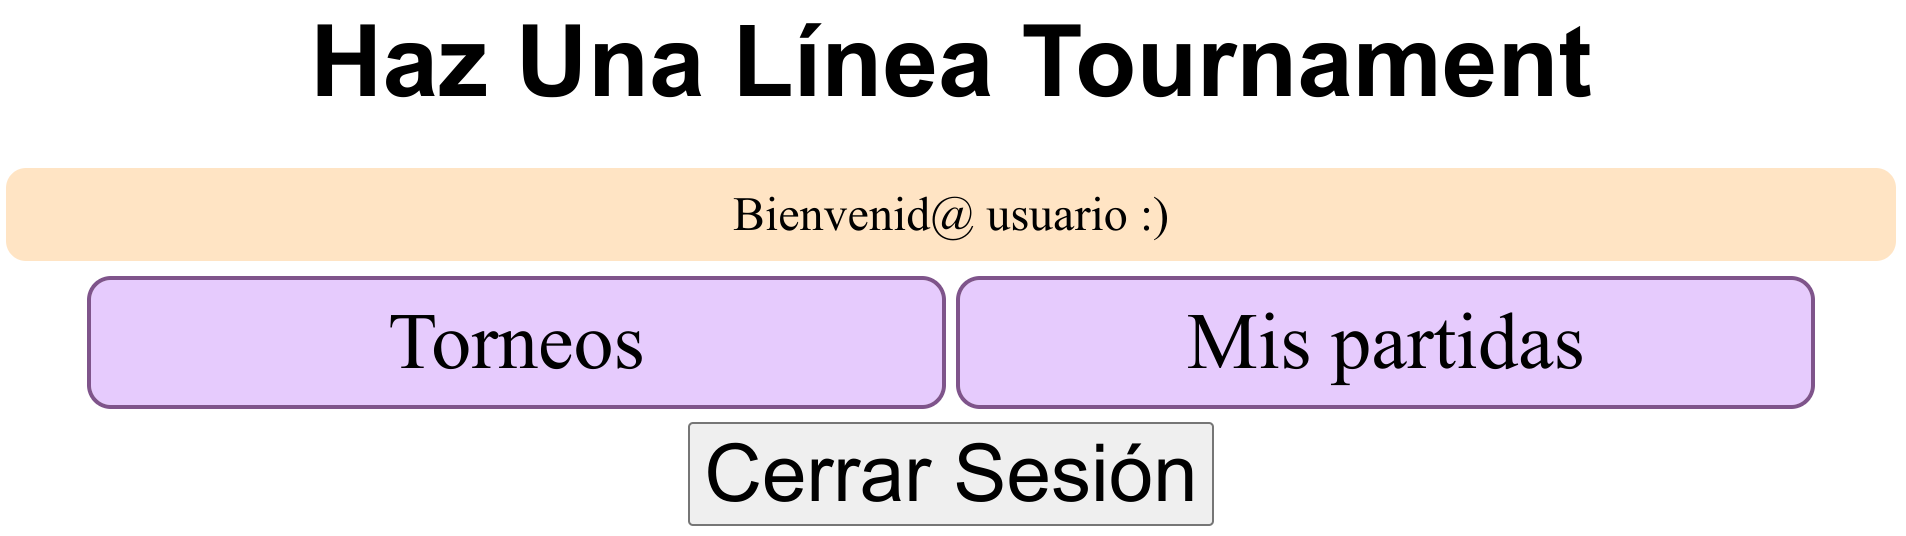
\includegraphics[width=\textwidth]{imagenes/inicioUser.png}
  \caption{Página de inicio del usuario no administrador} 
\end{figure}

\begin{figure}[H]
  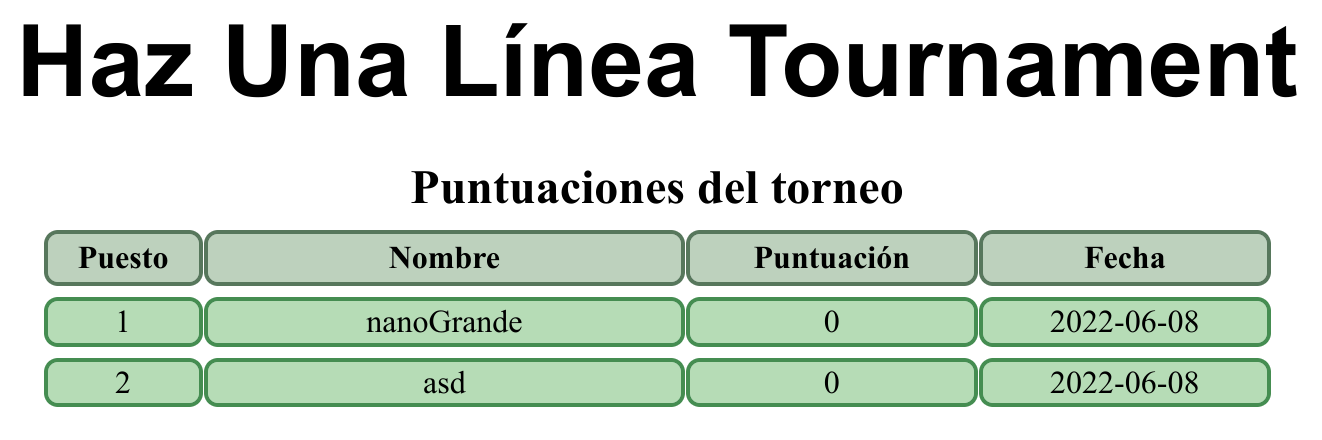
\includegraphics[width=\textwidth]{imagenes/torneoPuntuacion.png}
  \caption{Clasificación de un torneo} 
\end{figure}

\begin{figure}[H]
  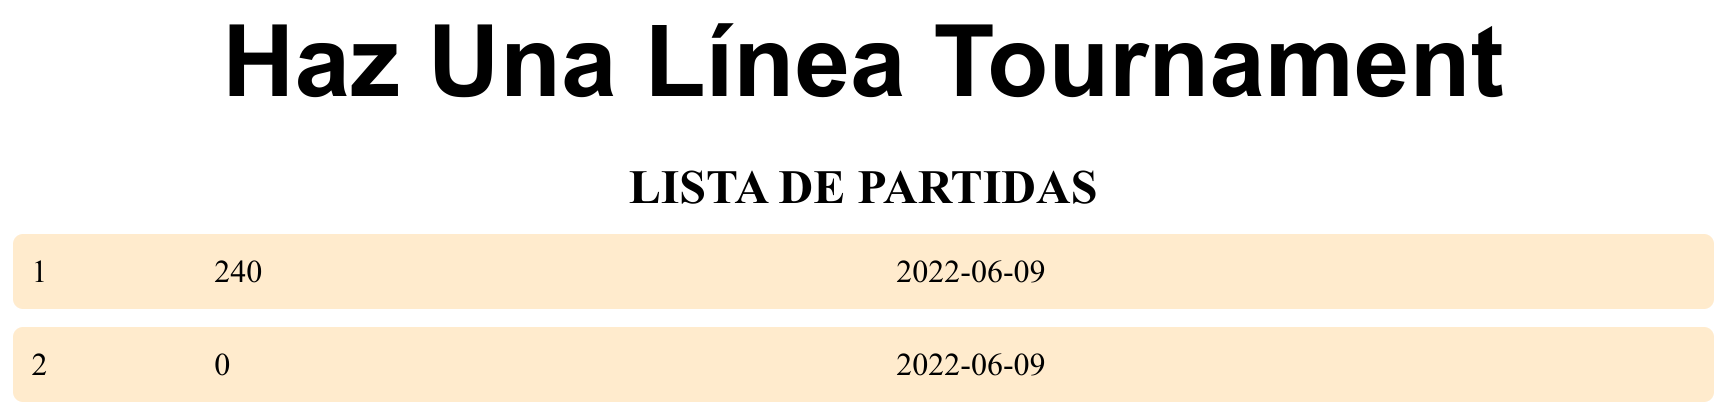
\includegraphics[width=\textwidth]{imagenes/puntuacion.png}
  \caption{Puntuaciones de partidas individuales de un usuario} 
\end{figure}

\begin{figure}[H]
  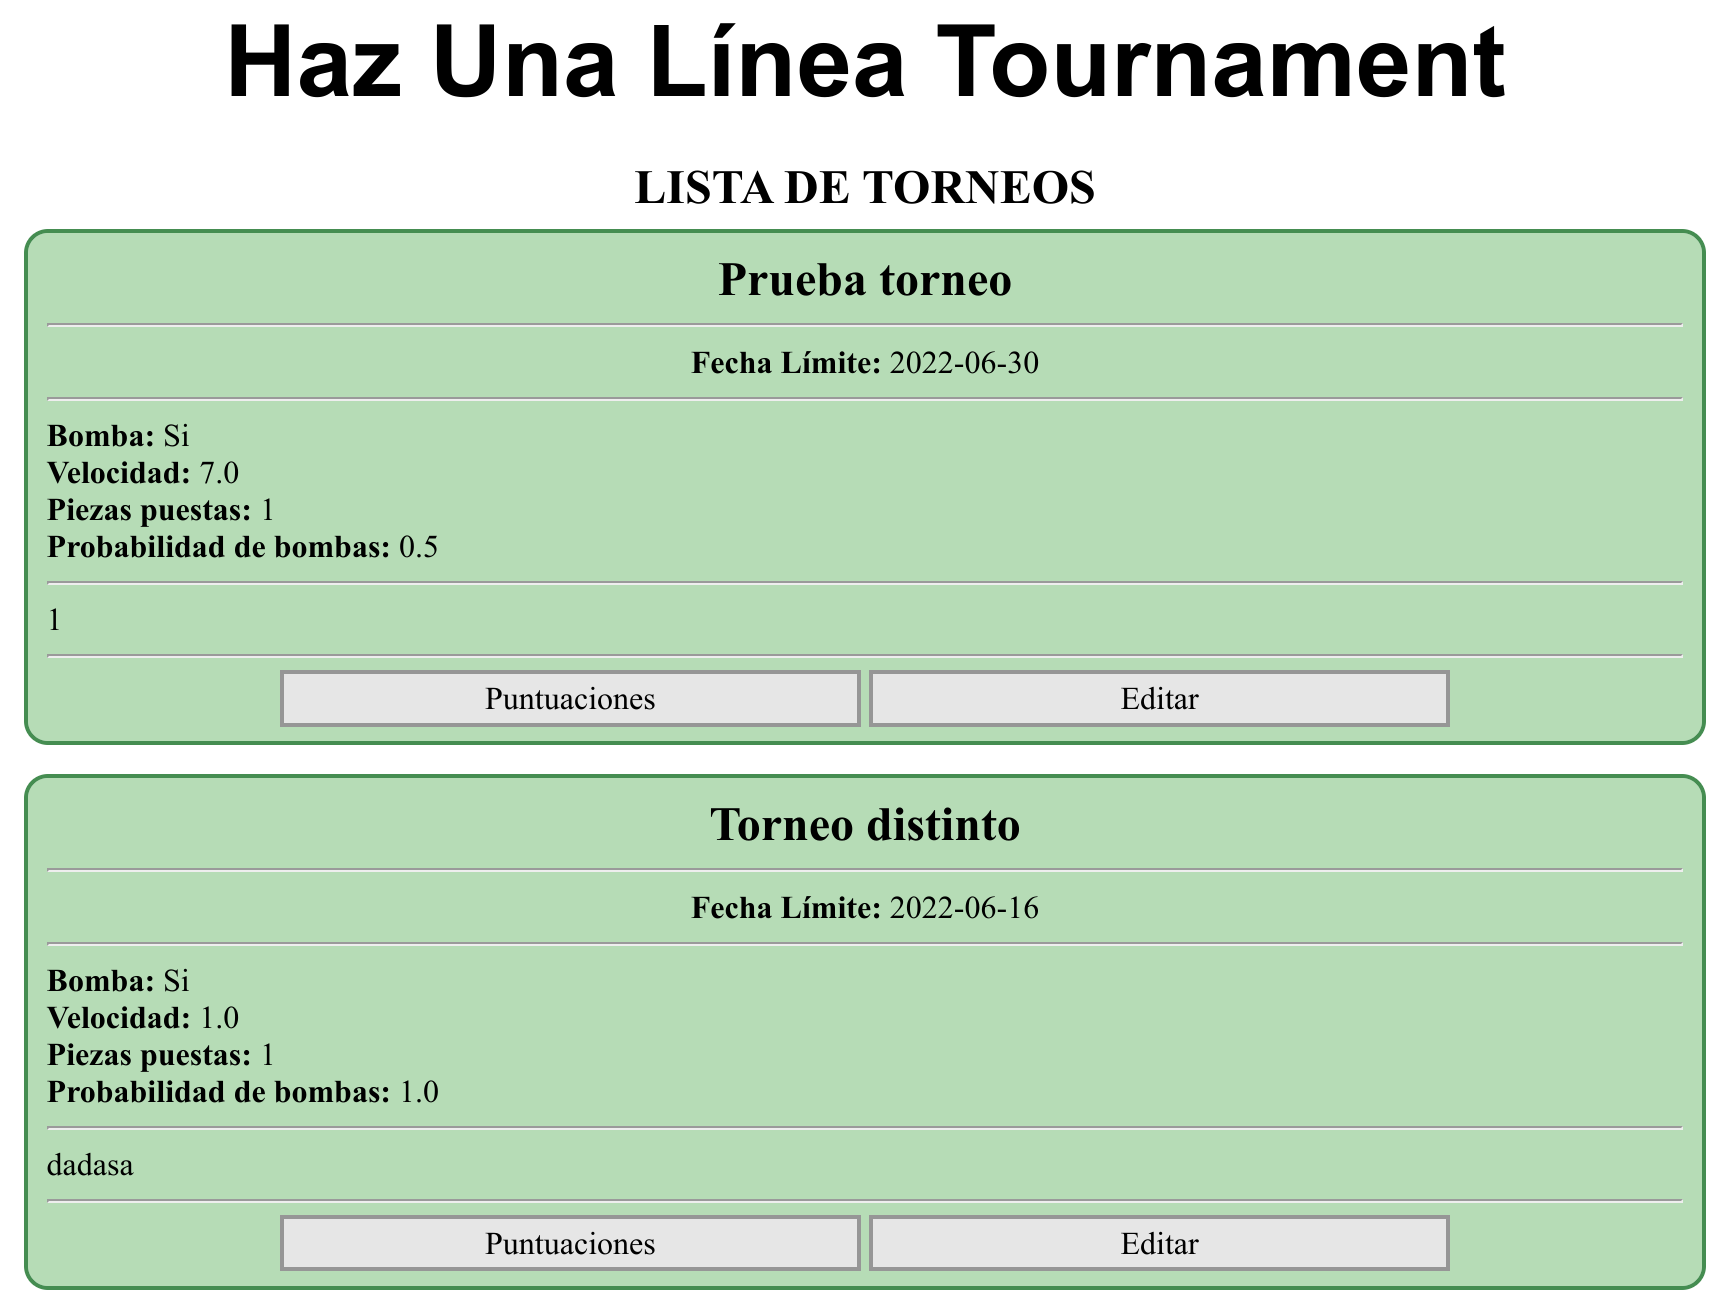
\includegraphics[width=\textwidth]{imagenes/adminTorneos.png}
  \caption{Lista de torneos vista desde el administrador} 
\end{figure}

\begin{figure}[H]
  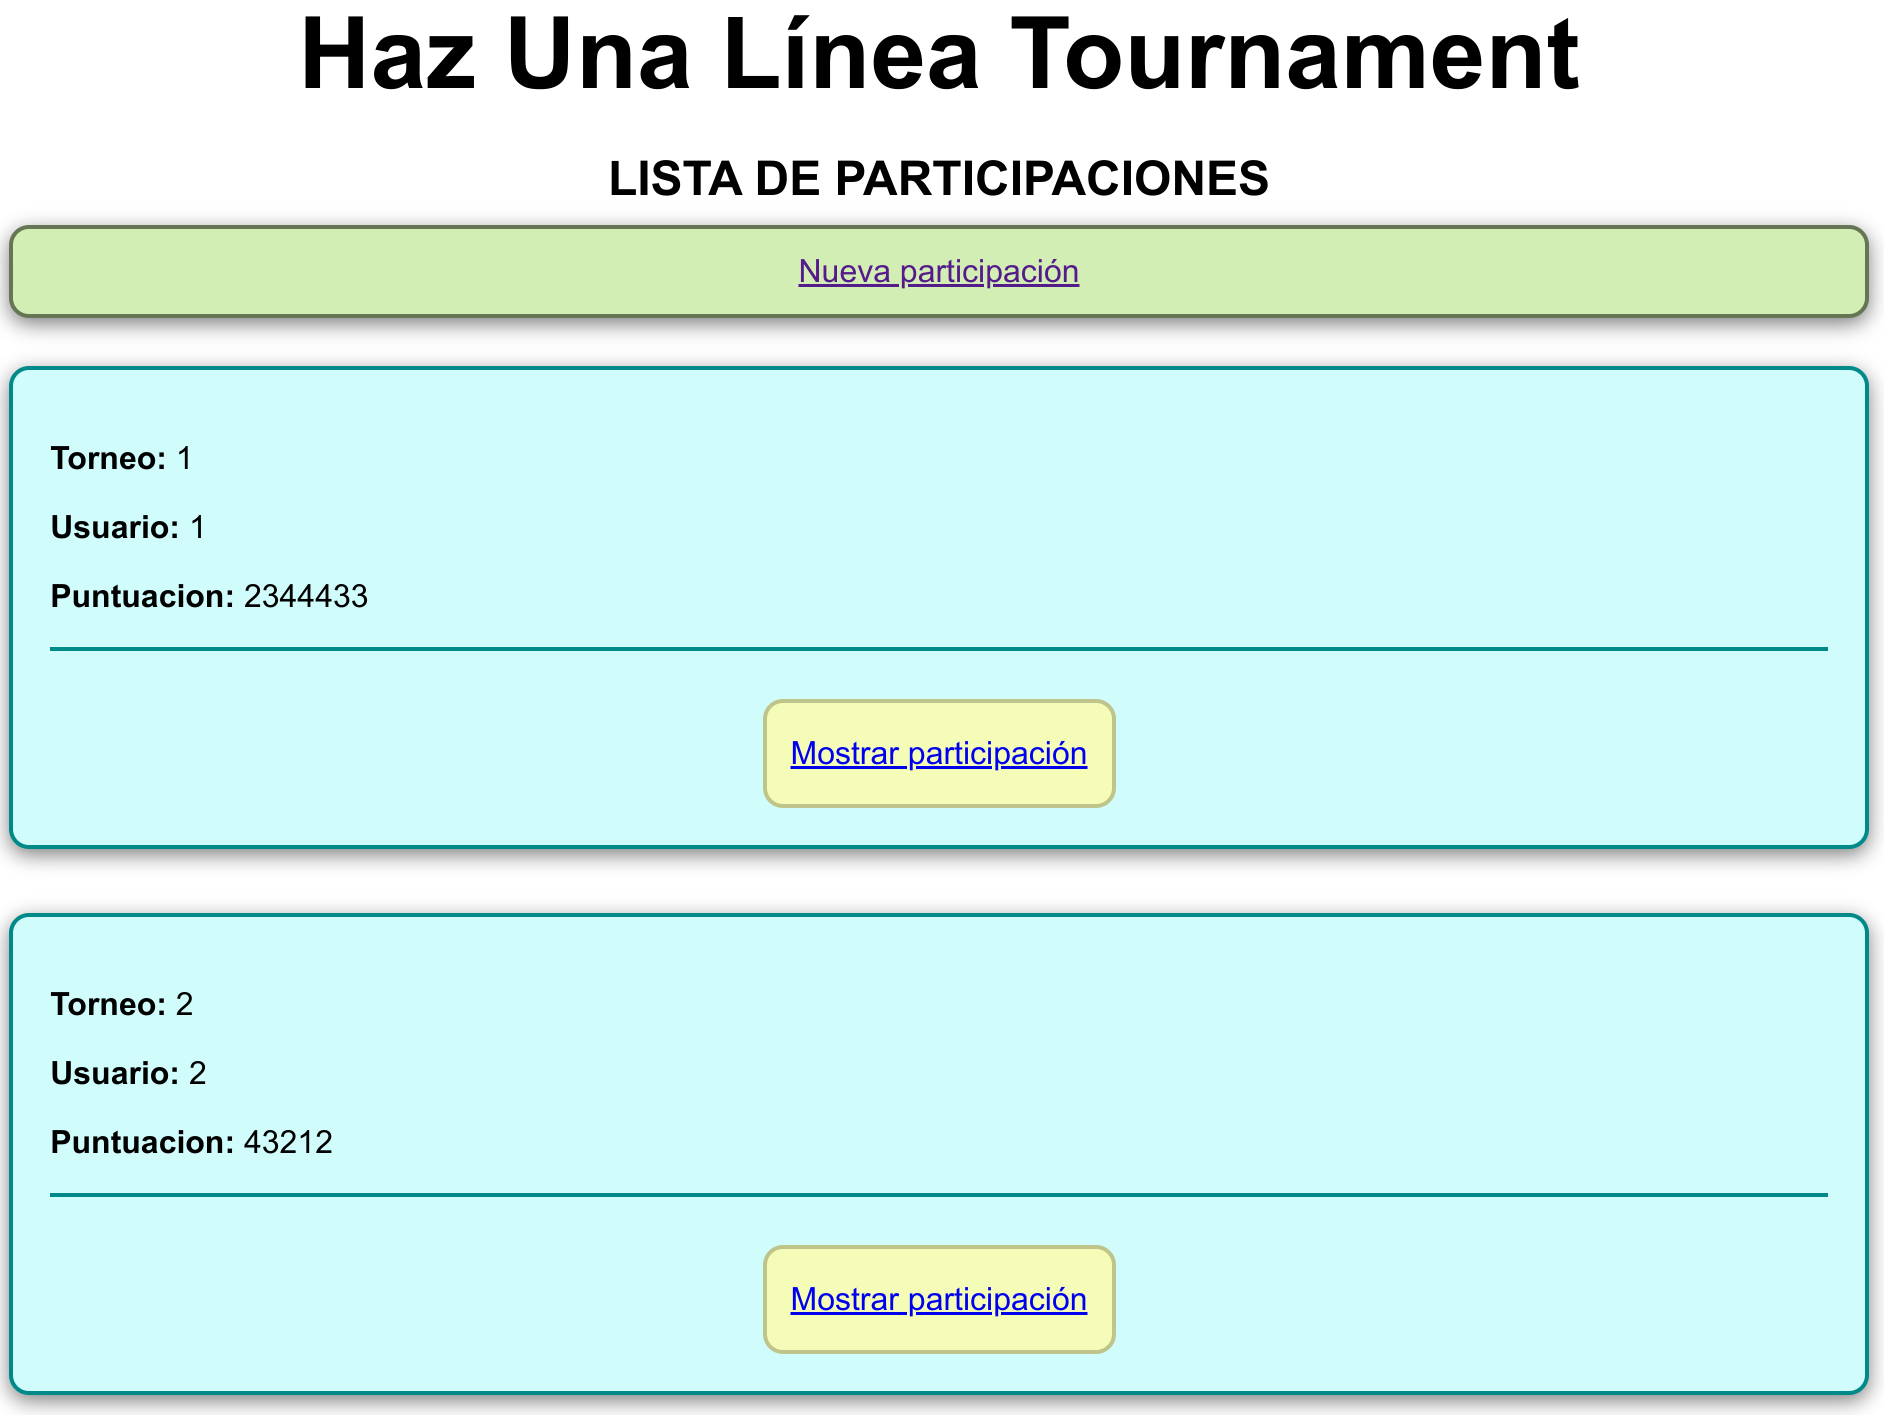
\includegraphics[width=\textwidth]{imagenes/adminPart.png}
  \caption{Gestión de las participaciones} 
\end{figure}

\begin{figure}[H]
  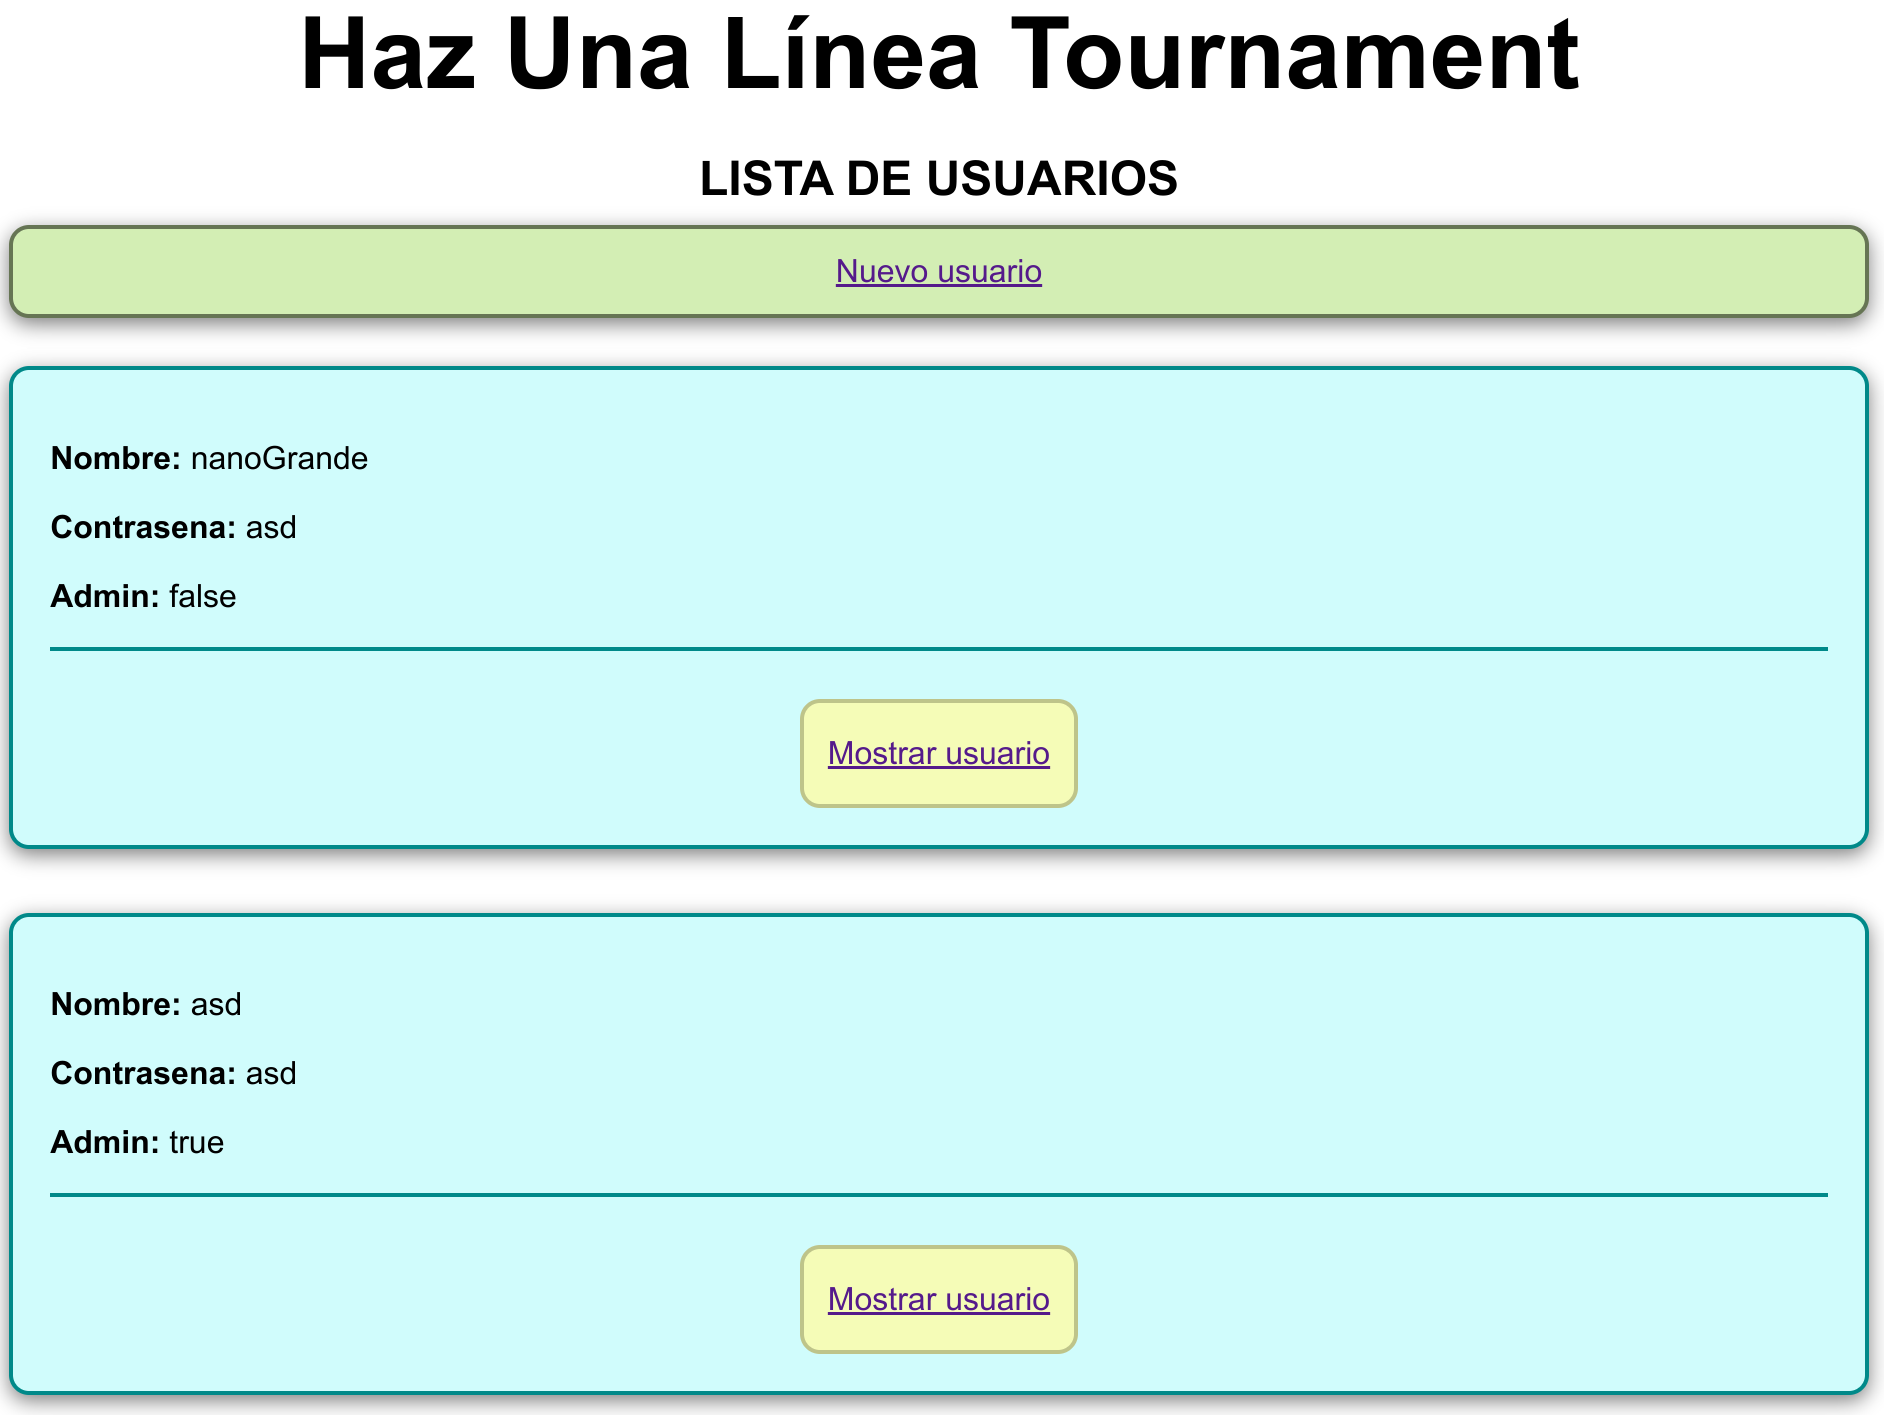
\includegraphics[width=\textwidth]{imagenes/adminUsers.png}
  \caption{Gestión de los usuarios} 
\end{figure}

\section{Conclusiones}
Para finalizar, tenemos que decir que nos ha parecido una práctica muy interesante, pues por fín hemos podido implementar una aplicación que parece
realmente útil y que se asemeja a lo que vemos día a día en nuestros dispositivos móviles. Pese a que la conexión con el servidor web nos ha costado más
de lo que creíamos y pese a no haber tenido el tiempo suficiente por otras materias, creemos que hemos hecho un buen trabajo en general para esta práctica ya que
hemos dotado de una funcionalidad a nuestro videojuego realmente interesante y original. 
\end{document}
